% build instructions:
% $> pdflatex thesis
% $> biber thesis
% $> pdflatex thesis
% $> pdflatex thesis
%
%
% J. Garofoli //  April 2014
\documentclass[hidelinks,letterpaper,12pt,oneside]{book}
% change to twoside for paper printing version

\linespread{2}
% su style guidelines
% http://www.syr.edu/gradschool/em/pdfs/emdissertation/Doctoral%20Dissertation%20%20Masters%20theses%20Format%20Guidelines.pdf
% https://en.wikipedia.org/wiki/Book_design

%\usepackage[T1]{fontenc}
\usepackage[hidelinks]{hyperref}
\usepackage{xcolor}
\hypersetup{
    colorlinks,
    linkcolor={red!50!black},
    citecolor={blue!50!black},
    urlcolor={blue!80!black}
}
\usepackage{ifthen}
\newboolean{uprightparticles}
\setboolean{uprightparticles}{false} %True for upright particle symbols

\newboolean{isdraft}
\setboolean{isdraft}{false} % change to false when final version is ready

\usepackage{xspace}
\usepackage{adjustbox} % for clipping seal images in xelatex
\usepackage{sidecap}
\usepackage{rotating} % for sidewaysfigure

\usepackage[english]{babel}
\usepackage[mdyy]{datetime}
\usepackage[margin=1in]{geometry}
\usepackage{everysel}
\usepackage{amsmath,amssymb}
%\usepackage[nomarkers]{endfloat}
%\usepackage{bm}
\usepackage{bookmark}
\usepackage[all]{hypcap} 
%\usepackage{feynmf}
\usepackage[nottoc]{tocbibind}
\usepackage{appendix}
\usepackage{color}
\usepackage{tabu}
\usepackage{xfrac}
\usepackage{paralist}

\usepackage{tikz}
\usetikzlibrary{arrows,decorations.pathmorphing,backgrounds,positioning,fit,petri,decorations.markings,patterns,plotmarks,shapes}
\usepackage{nomencl}
\makenomenclature
\renewcommand{\nomname}{List of Abbreviations}

% if using xelatex, will also format math
%\usepackage[Numbers=OldStyle,Ligatures=TeX,Scale=MatchLowercase]{mathspec}
%\setallmainfonts{Source Sans Pro Light}
%\newfontfamily\semibold{Source Sans Pro}
%\newcommand\tracked[1]{{\addfontfeature{LetterSpace=12}#1}} % for all caps words
%\usepackage{xunicode}
%\defaultfontfeatures{Mapping=tex-text}
%\usepackage{unicode-math}
%\usepackage{hvmath}
%\usepackage[Euler]{upgreek}

%\usepackage[default,light,oldstyle,semibold]{sourcesanspro}
%\usepackage[cmbright]{sfmath}

\usepackage[tracking=true]{microtype}
\SetTracking
 [ no ligatures = {f},
 spacing = {600*,-100*, },
 outer spacing = {450,250,150},
 outer kerning = {*,*} ]
 { encoding = * }
 { 160 }
\newcommand\tracked[1]{\textls{#1}}


%\usepackage[default]{sourcesanspro} % doesn't change some any greek letters (only pi and o)
%\usepackage{microtype} % doesn't really work with xelatex
%\usepackage{sfmath}

\usepackage[font={it}]{caption}
\captionsetup[table]{aboveskip=12pt}
\captionsetup[table]{belowskip=12pt}



\usepackage[center]{titlesec}
\titleformat{\part}[display]{\Huge\filcenter\normalfont}{Part \thepart\\}{0pt}{\Huge\normalfont}
\titleformat{\chapter}[display]{\large\filcenter\normalfont}{\color{gray} Chapter \thechapter}{0pt}{\huge\normalfont}
\titleformat{\section}{\normalfont\filcenter\large}{\thesection}{1em}{}
\titleformat{\subsection}{\normalfont\filcenter\large}{\thesubsection}{1em}{}
\titleformat{\subsubsection}[runin]{\normalfont\scshape}{\thesubsubsection}{1em}{}[:]
\titleformat{\paragraph}[runin]{\normalfont\itshape}{\theparagraph}{}{}[:]
\titlespacing{\paragraph}{0em}{0em}{0.2em}
\usepackage{titletoc}

\usepackage{tocloft}
\renewcommand{\cftpartfont}{\Large \normalfont}
\renewcommand{\cftpartpagefont}{\large \normalfont}
\renewcommand{\cftchapfont}{\large \normalfont}
\renewcommand{\cftchappagefont}{\large \normalfont}
\renewcommand{\cfttoctitlefont}{\huge \normalfont}
\renewcommand{\cftloftitlefont}{\huge \normalfont}
\renewcommand{\cftlottitlefont}{\huge \normalfont}
%\makeatletter
%\renewcommand{\@numwidth}{2.55em}
%\makeatother

\frenchspacing
\usepackage{parskip}
\setlength{\parskip}{0.35cm}
\usepackage{setspace}
%\onehalfspace
\doublespace

\usepackage{sparklines}

\ifthenelse{\boolean{isdraft}}{
\usepackage{lineno}
\linenumbers
% there is a problem with amsmath and lineno stuff, so here is a fix
% from http://phaseportrait.blogspot.com/2007/08/lineno-and-amsmath-compatibility.html
\newcommand*\patchAmsMathEnvironmentForLineno[1]{%
  \expandafter\let\csname old#1\expandafter\endcsname\csname #1\endcsname
  \expandafter\let\csname oldend#1\expandafter\endcsname\csname end#1\endcsname
  \renewenvironment{#1}%
     {\linenomath\csname old#1\endcsname}%
     {\csname oldend#1\endcsname\endlinenomath}}% 
\newcommand*\patchBothAmsMathEnvironmentsForLineno[1]{%
  \patchAmsMathEnvironmentForLineno{#1}%
  \patchAmsMathEnvironmentForLineno{#1*}}%
\AtBeginDocument{%
\patchBothAmsMathEnvironmentsForLineno{equation}%
\patchBothAmsMathEnvironmentsForLineno{align}%
\patchBothAmsMathEnvironmentsForLineno{flalign}%
\patchBothAmsMathEnvironmentsForLineno{alignat}%
\patchBothAmsMathEnvironmentsForLineno{gather}%
\patchBothAmsMathEnvironmentsForLineno{multline}%
}
}{ % no line numbers for not a draft
    }

\usepackage{fancyhdr}

\setlength{\headheight}{15pt}
\fancypagestyle{plain}{%
\fancyhf{} % clear all header and footer fields
\ifthenelse{\boolean{isdraft}}{
\fancyhead[LO,RE]{\small - * - \tracked{DRAFT} \today~- * -}
}{}
\fancyhead[RO]{\small \tracked{\scriptsize \leftmark}\hspace{3mm}\thepage} % except the center
\renewcommand{\headrulewidth}{0pt}
\renewcommand{\footrulewidth}{0pt}
\renewcommand{\headheight}{16pt}
\fancyhead[LE]{\small \thepage\hspace{3mm}\tracked{\scriptsize \leftmark}} % except the center
\renewcommand{\headrulewidth}{0pt}
\renewcommand{\footrulewidth}{0pt}
\renewcommand{\headheight}{16pt}}

\fancypagestyle{plainbottom}{%
\fancyhf{} % clear all header and footer fields
\ifthenelse{\boolean{isdraft}}{
\fancyhead[LO,RE]{\small - * - \tracked{DRAFT \today}~- * -}
}{}
\fancyfoot[C]{\small \thepage} % except the center
\renewcommand{\headrulewidth}{0pt}
\renewcommand{\footrulewidth}{0pt} }

\fancypagestyle{empty}{%  just delete this when not in draft any more
\fancyhf{} % clear all header and footer fields
\ifthenelse{\boolean{isdraft}}{
\fancyhead[LO,RE]{\small - * - \tracked{DRAFT \today}~- * -}
}{}
\renewcommand{\headrulewidth}{0pt}
\renewcommand{\footrulewidth}{0pt}}

\pagestyle{plainbottom}





%% from http://tex.stackexchange.com/questions/22100/the-bar-and-overline-commands
\makeatletter
\newsavebox\myboxA
\newsavebox\myboxB
\newlength\mylenA
\newcommand*\xoverline[2][0.75]{%
    \sbox{\myboxA}{$\m@th#2$}%
    \setbox\myboxB\null% Phantom box
    \ht\myboxB=\ht\myboxA%
    \dp\myboxB=\dp\myboxA%
    \wd\myboxB=#1\wd\myboxA% Scale phantom
    \sbox\myboxB{$\m@th\overline{\copy\myboxB}$}%  Overlined phantom
    \setlength\mylenA{\the\wd\myboxA}%   calc width diff
    \addtolength\mylenA{-\the\wd\myboxB}%
    \ifdim\wd\myboxB<\wd\myboxA%
       \rlap{\hskip 0.5\mylenA\usebox\myboxB}{\usebox\myboxA}%
    \else
        \hskip -0.5\mylenA\rlap{\usebox\myboxA}{\hskip 0.5\mylenA\usebox\myboxB}%
    \fi}
\makeatother

%% from http://tex.stackexchange.com/questions/109576/change-sqrt-symbol 
%\def\radice#1{\surd\kern-.25pt\overline{\mathstrut#1}}

%\makeatletter
%\let\ps@plain\ps@fancy
%\makeatother
\AtBeginDocument{\addtocontents{toc}{\protect\thispagestyle{plainbottom}}}
\AtBeginDocument{\addtocontents{lof}{\protect\thispagestyle{plainbottom}}}
\AtBeginDocument{\addtocontents{lot}{\protect\thispagestyle{plainbottom}}}

\DeclareTextCommandDefault{\nobreakspace}{\leavevmode\nobreak\ }

\DeclareGraphicsRule{*}{mps}{*}{}

\usepackage{stmaryrd}
\renewcommand\to{\rightarrowtriangle}
\renewcommand\rightarrow{\rightarrowtriangle}

\newcommand{\avg}[1]{\left< #1 \right>} % for average

\renewcommand\labelitemi{\small$\square$}

%\addto\captionsenglish{\renewcommand{\bibname}{References}}

\usepackage[hyperref=true,
            url=true,
            isbn=false,
            backref=true,
            style=numeric-comp,
            maxcitenames=3,
            maxbibnames=100,
            sorting=none,
            arxiv=abs,
            block=none]{biblatex}
\addbibresource{thesis.bib}
\DefineBibliographyStrings{english}{%
  bibliography = {References},
}

\renewcommand{\bibsetup}{\pagestyle{plain}}



%\input{/Users/justing/jgarofol/analysis/B2Dkpipi/Restrip/ana/mylatexvars2}
%\input{mylatexvars2}

\begin{document}
\setlength{\unitlength}{1mm}
\frontmatter
\pagestyle{plainbottom}

\begin{center}
\tracked{ABSTRACT}\\[12pt]
%\updateme
\end{center}
\vspace*{2cm}
\linespread{2}
%\addcontentsline{toc}{chapter}{Abstract}
Early developmental disorders are common in children between the ages of 3 through 17. These developmental disorders begin at early ages and affect the day-to-day activity of children. They also impact the growth and lifestyle of children. Most of the time these developmental disorders co-exist in children. The main focus of our research lies in the disorders `Autism Spectrum Disorder', `Attention-Deficit/Hyperactivity Disorder', `Deletion syndrome (22q)' and their co-occurrences.

Most child psychologists and pediatricians diagnose these disorders in children through parent-oriented reviews. Our research uses three different parent-oriented reviews, which are `Autism Diagnostic Interview', `Behavioral Assessment Schedule for Children', and `Vineland Adaptive Behavior Scales'. These reviews are questionnaires that parents answer under the inspection of certified professionals. While these examinations take up lots of time and yield results after at least 13 months of wait time, the process needs to speed up and hence, machine learning could play a vital role in this process.

Machine learning, when applied to reviews, can help understand the relevance and importance of them in diagnosing the disorders. Also, many techniques have been applied in our research to evaluate the co-occurrence of these disorders. The objective is to determine if machine learning could predict the occurrence of these disorders. Also, decide the significance of these reviews using feature selection algorithms of machine learning.
\setcounter{page}{1}
\thispagestyle{empty}
\pagestyle{empty}
\cleardoublepage

%\title{\bf Study of the Decays\\
%\boldmath{$B^- \rightarrow D^0 K^- \pi^+ \pi^-$},\\
%\boldmath{$D^0 \rightarrow K^+\pi^-, K^+K^-, \pi^+\pi^- \text{ or } K^-\pi^+$}}
%
%% alternative:
%% The Measurement of the CP Violation Paramters in
%% The Decay ....
%
%\author{by\\[10pt]
%    JUSTIN GAROFOLI\\[10pt]
%Bachelor of Science\\
%Western Washington University\\
%Bellingham, Washington, 2001 }
%
%\date{
%    Syracuse University\\[10pt]
%    \today}
%
%\maketitle

\begin{titlepage}
\begin{center}
\vspace*{0.2cm}
\noindent\makebox[\linewidth]{\rule{\textwidth}{0.3pt}}
{\huge %[Update Title]\\
Computational Analysis of Developmental Disorders in Children\\[0.4cm]
}
\noindent\makebox[\linewidth]{\rule{\textwidth}{0.3pt}}\\ % fix spacing here
\vspace{0.5cm}
%by (fix spacing above and at top)\\
\vspace{0.5cm}
\tracked{\large Siri Chandana~ Sambatur}\\[6pt]
Bachelor of Technology\\
VNR Vignana Jyothi Institute of Engineering and Technology\\
Telangana, (India) 2016\\
\vspace{1.3cm}
\tracked{\large DISSERTATION}\\[6pt]
Submitted in partial fulfillment\\
of the requirements for the degree\\
\emph{Master of Science in Computer Science}\\
\ifthenelse{\boolean{isdraft}}{
\vspace{1cm}
- * - \tracked{DRAFT \today}~- * -\\[0.5cm]
}{
\vspace{1.5cm}
}
May, 2018\\
Syracuse University\\
Syracuse, New York
%SYRACUSE UNIVERSITY MMXIII

\end{center}
%\setcounter{page}{2}
\end{titlepage}

\vspace*{5cm}
\begin{center}
    Copyright \textcopyright Siri Chandana Sambatur 2018\\
    All Rights Reserved\\
    %Syracuse University\\
\end{center}
\setcounter{page}{3}
\thispagestyle{empty}

\clearpage

%\begin{center}
%\vspace*{3cm}
%\includegraphics[width=0.95\textwidth]{figs/leman-alps-sky}
%\thispagestyle{empty}
%\end{center}

%\input{committee}
\pagestyle{plainbottom}
%\titleformat{\section}
 % {\normalfont\Large\bfseries}{\thesection}{1em}{}[{\titlerule[0.8pt]}]
\section*{Acknowledgments}

I am grateful to my advisor, Dr. Reza Zafarani of the Department of EECS at
Syracuse University. He guided me throughout my research and helped me overcome various obstacles that I faced. Dr. Zafarani directed me in the right path during my research and advised of various prospective areas to explore. Along with Dr. Zafarani, Dr. Russo helped me understand the psychological aspects of my research. I am thankful to them for the encouragement and constant support.

I would also like to thank the experts who were involved in the Defense Committee without whose participation,  the Defense could not have been successfully conducted:
\begin{itemize}
\item Dr. Natalie Russo, Assistant Professor, Department of Psychology
\item Dr. Senem Velipasalar Gursoy, Associate Professor, Department of Electrical Engineering and Computer Science
\item Dr. Edmund Yu, Associate Professor, Department of Electrical Engineering and Computer Science
\end{itemize}

I would like to give credit to my parents Mamatha and Gowri Shankar Sambatur, my brother Abhishek Shankar for always motivating me. Also, I would like to thank my friends Sai Venkat Kotha, Ayesha Ahmad and Rashmi K. Shivanna, who supported and rooted for me during this journey. Finally, I am also grateful to my laboratory mates who assessed and advised on various aspects of my thesis. This accomplishment would not have been possible without all these people. 

\hfill\emph{Sambatur, Siri Chandana}\\
\hspace*{0pt}\hfill\emph{Syracuse, New York}\\
\hspace*{0pt}\hfill\emph{May, 2018}


\pagestyle{plainbottom}
\addtocontents{toc}{\protect{\pdfbookmark[0]{\contentsname}{toc}}}
\tableofcontents
\clearpage
\listoffigures
\clearpage
\listoftables
\cleardoublepage
\printnomenclature 

\pagestyle{empty}
\cleardoublepage
\mainmatter
\renewcommand{\chaptermark}[1]{\markboth{\MakeUppercase{#1}}{}}
\pagestyle{plain}
% perhaps put introduction in the front matter
% and have three chapters of 1) current understanding
%                            2) experimental considerations
%                            3) theoretical motivation
% decide later, do the writing first
\chapter{Introduction}
%\addcontentsline{toc}{chapter}{Introduction}
\thispagestyle{plainbottom}
Most children suffer from different kinds of developmental disorders. Among the many disorders present, the most common ones are ASD, ADHD and VCFS. While VCFS is a genetic defect, the causes of ASD and ADHD are not known. There various studies in this field to identify the genetics behind these two disorders. Also, few children suffer from more than one disorder and sometimes one leads to another. Therefore, it is essential to understand as much about these developmental disorders as possible.

Clinicians take almost 13 months to diagnose children and even later in the case of comorbid disorders. Many researchers have developed techniques for early intervention of these disorders. As these disorders effect the trajectory of growth of children, early intervention is critical for children and families to led normal lives. A lot of researchers believe that machine learning could speed up this process and play a vital role in early diagnosis. So, the main aim of our research is to analyze these disorders, understand them better and try to build models for prediction of these disorders. Our key contributions are as follows-
\begin{itemize}
\item Identifying important features for developmental disorders ASD, VCFS and ADHD, along with the comorbid disorders.
\item Assessing the impact of the three different parent-oriented reviews on these developmental disorders and their comorbidity.
\item Designing models to diagnose these different subgroups of developmental disorders present in the data
\item Designing models to diagnose for the comorbid disorders `ASD and VCFS' and `ASD and ADHD'
\item Designing models for each individual diagnosis that is ASD, VCFS and ADHD.
\item Formulating hypothesis using the features relation found in our models to assess the developmental disorders
\end{itemize}


Initially, in our thesis, more information is provided on these developmental disorders and their comorbidity. The parent-oriented reviews which will be used for our data are explained. Also, in chapter 2, the various models that have been designed using machine learning to diagnose these disorders are explained. Before applying machine learning on our data, in chapter 3, the data is analyzed and preprocessed. Furthermore, analysis and observations are made on the significant features related to these developmental disorders. Later on in chapter 4, understanding of various subgroups in our data is done using both unsupervised and supervised techniques. Additional information on the comorbidity of the disorders is examined in chapter 5 and finally, in chapter 6, each of these individual developmental disorders are investigated. 



\linespread{2}
\chapter{Related Work}
%\addcontentsline{toc}{chapter}{Introduction}
\thispagestyle{plainbottom}
Developmental Disorders comprise of a group of psychiatric conditions that originate in childhood and cause severe problems in certain areas. According to the Centers for Disease Control and Prevention (CDC), more than one out of every 100 school children in the United States has some form of mental retardation. The third most common disorder is Autism Spectrum Disorder.
\nomenclature{ASD}{Autism Spectrum Disorder}Developmental disorders are caused because of various reasons like genetics (Deletion syndrome) or due to complications in pregnancy or birth. However, most of the times the exact causes are not known. It can also be seen that developmental disorders are common occurrences in children when the mother goes through stress or consumes alcohol during pregnancy~\cite{webpage2}. For proper livelihood of the child, early identification of these disorders is crucial as their causes could be reversed. Most children who were diagnosed with ASD usually reported initial signs of concern before the child was 2 years old in their records. However, most of these children were diagnosed only after age 4, almost 82\% of the time by age 3 and 21\% of the time at 8 years ages\cite{christensen2016prevalence}. Early identification helps families to prepare strategies and other resources for successful families. 

The occurrence of multiple disorders causes more complexity in identifying them as one of those disorders would be diagnosed and the other would take more time to identify. Children who are diagnosed with ASD could also be suffering from ADHD\nomenclature{ADHD}{Attention Deficit/Hyperactivity Disorder} or vice-versa. The relationship between these two disorders is still debated in the field of psychology. While children suffering from VCFS\nomenclature{VCFS}{22q Deletion Syndrome} could also be affected with Schizophrenia. It was observed that 2 in every 178 patients suffering from Schizophrenia had VCFS~\cite{bassett199922q11}. Also, a study done with data collected from a congenital cardiac clinic reported that 22.6\% of adults with VCFS had schizophrenia or schizoaffective disorder~\cite{bassett2005clinical}. 

Machine learning could help build models to analyze these causes much faster and help in speeding up the diagnosis process. With this research, we hope to identify the causes for single or multiple disorders with our models with good accuracies and also differentiate subjects based on different features. While machine learning algorithms seem to be showing promising results, there could be some pitfalls. It is essential that when applying these techniques the researchers should be made aware of all aspects of the study as this is an interdisciplinary research and some of these issues like methodology and implementation are discussed by author Wall ~\cite{wall2012use}. Further details about the relationship between these diseases are essential for our knowledge and hence, will be discussed before understanding how machine learning is playing a crucial role.
\section{Developmental Disorders and Comorbidity}
While most developmental disorders deal with mental retardation, Autism Spectrum Disorder(ASD) is characterized by social interaction difficulties and communication challenges. There are many types of autism which are caused by different genetic combinations and environmental influences. The Centers for Disease Control and Prevention (CDC) estimates that it is present in 1 out of 68 children in the United States. It seems to occur 4.5 times more frequently in boys than girls. The four sub-types of Autism are Autistic Disorder, Asperger’s Syndrome, Childhood Disintegrative Disorder and Pervasive Developmental Disorder according to the fourth edition of Diagnostic and Statistical Manual of Mental Disorders(DSM) which is published by American Psychiatric Association(APA). However, in the fifth edition published in 2013, all of these four sub-types were dissolved into a single disorder called Autism Spectrum Disorder and the American Psychiatric Association(APA) felt that it this would be helpful for accurately diagnosing individuals with autism~\cite{edition2013diagnostic}. 

Attention-Deficit/hyperactivity disorder(ADHD) is also a brain disorder with patterns of inattention and/or hyperactivity that affects the development of a child. Children who suffer from ADHD have difficulty in staying focused and paying attention, and difficulties with controlling behavior. Similar to ASD, ADHD also seems to have more prevalence among male children~\cite{visser2014trends}. This disorder also continues to affect the children in their adulthood, almost one-third of children diagnosed with ADHD retain it even in adulthood~\cite{barbaresi2013mortality}. According to the fourth edition of Diagnostic and Statistical Manual of Mental Disorders, published in 2000 by APA, there are three sub-types of ADHD. The three sub-types are combined type of ADHD, predominantly inattentive type ADHD and predominantly hyperactive-impulsive type ADHD. Both ASD and ADHD are disorders for which the causes are not clear and also researchers are not sure about the role played by environmental factors.

Deletion syndrome 22q11.2(VCFS) is also known as DiGeorgesyndrome as it was first described by Angelo DiGeorge in 1968~\cite{digeorge1968congenital,restivo200622q11}. It is caused by the deletion of 30 to 40 genes in the middle of chromosome 22 at a location known as 22q11.2. This is a genetic disorder and 10\% of the cases are inherited by a parent. DiGeorge syndrome occurs in about 1 in 4,000 people. Children diagnosed with this disease have delayed growth and speech development, and also have learning disabilities. Individuals affected by this disorder have breathing problems, low levels of calcium in blood and kidney abnormalities. Unlike ASD and ADHD, VCFS can be diagnosed by performing genetic analysis to detect microdeletions. Fluorescencein situhybridization(FISH)is a method which helps diagnose VCFS, quantitative polymerase chain reaction(qPCR) is quicker than FISH. It has a turn around time of 3 to 14 days. Those affected by VCFS have the risk of developing other disorders like schizophrenia, depression, anxiety, and bipolar disorder~\cite{mcdonald2011chromosome}.

While each of these disorders affects a person in a different way they are also related to one another or more specifically one leads to another. When these disorders co-occur then they are called comorbid disorders. As mentioned earlier ASD and ADHD which co-occur are comorbid disorders while VCFS and schizophrenia are comorbid disorders. It is essential to understand their comorbidity to better analyze and diagnose these disorders.
\subsection{Co-occurrence of VCFS and Schizophrenia}
Schizophrenia is also a mental disorder where the diagnosed fail to understand reality and lack of normal social behavior. People with schizophrenia have unclear thoughts, anxiety, depression and reduced social engagement~\cite{cross2017external} ~\cite{webpage1}. The evidence for VCFS being the first identifiable genetic subtype of schizophrenia was given by Anne. S. Bassett~\cite{bassett2008schizophrenia}. In this research, it was found that individuals whose relatives have schizophrenia tend to have a lower probability of containing individuals with 22qDS. Most studies that were done with different samples of data show that the relative risk for schizophrenia in an individual initially diagnosed with 22qDS is about 20 to 25 times the lifetime general population risk of 1\% ~\cite{bassett2000chromosomal}~\cite{hodgkinson2001genetic}.

When a study was conducted on non-overlapping samples, in which 82 individuals had VCFS and schizophrenia showed some comparable clinical signs~\cite{bassett2008schizophrenia}. By comparing the IQ of the patients, some reports showed that the IQ was same that is ranged from 70-84 irrespective of whether the patient had schizophrenia or not~\cite{chow2006neurocognitive}. On the other hand, another study found mental retardation in 69\% patients, found lower IQ levels for patients with VCFS and schizophrenia than patients with no schizophrenia\cite{raux2006involvement}. Some other findings that distinguish these patients were that they had smaller brain volume, midline defects such as cavum septum pellucidum, and white matter hyper intensities on MRI~\cite{van2004brain}~\cite{chow1999qualitative}. 

Due to these studies being carried out even though most of the times it continues to be unrecognized, clinicians are educated of the possibilities during diagnosing individuals. This would help them look for signs of schizophrenia in patients with VCFS. Also, they could let patients known about possibilities of schizophrenia and other disorders too.
\subsection{Co-occurrence of VCFS and ASD}
According to research, 15-20\% patients diagnosed with VCFS meet the behavioral criteria for a diagnosis of ASD. Due to the missing DNA of the 22 chromosome,  there could be modifying affects in each person’s set of genes. Some individuals could have social difficulties, developmental delays or learning disabilities. These are some of the symptoms of an autistic child. Hence, it is believed that understanding genetic causes for autism is important.

Various studies have been conducted to examine the extent to which VCFS individuals also have ASD. One of these studies uses children, adolescents and young adults whose males to females ratio is 2.3:1. Based on the information from the Autism Diagnostic Interview-Revised (ADI-R), the Autism Diagnostic Observational Schedule (ADOS), and a clinician’s best-estimate diagnosis, they estimated that ASD is present in 15-50\% of the cases~\cite{ousley2017examining}.

By studying the phenotypes, differences with the children with VCFS and VCFS+ASD is being researched. From this analysis it was seen that 94\% of the children with VCFS + ASD had a co-occurring psychiatric disorder, on the other hand, 60\% of children with VCFS had a psychiatric disorder. Also, further studies of the brain showed that children with VCFS + ASD had larger right amygdala volumes and all other neuro-anatomic regions of interest were statistically similar between the two groups~\cite{antshel2007autistic}.

Apart from schizophrenia, ASD is also one of those psychiatric disorders that children with VCFS could possibly have. In our study, some analysis has been done to study the phenotypes of children with VCFS and VCFS+ASD using machine learning techniques. Techniques have mainly been applied to find distinguishable features and help broaden the understanding with the co-occurrence of these two developmental disorders.

\subsection{Co-occurrence of ASD and ADHD}
ASD and ADHD are two developmental disorders that affect an increasing number of children. These two developmental disorders share some common symptoms like lack of concern, not being able to react to others emotions or feelings etc. The reason why it is difficult to distinguish symptoms of ASD from ADHD is that they occur at the same time. In one of the studies in pediatrics field, showed that 18\% of the children diagnosed with ADHD showed signs of ASD~\cite{kotte2013autistic}. So, when this disorder occurs in children, they tend to have learning complications and impaired social skills.

Various studies have been done in the field of psychology to understand the relation between these two developmental disorders. However, researchers are still not certain about why these two developmental disorders occur together frequently. Initially, doctors never diagnosed a child with these two disorders, as they believed that they could not coexist as per the APA. It was in 2013, the release of the Diagnostic and Statistical Manual of Mental Disorders, Fifth Edition (DSM-5) when the APA stated that ASD and ADHD could co-occur~\cite{american2013diagnostic}. Researchers found that 20-50\% of the individuals diagnosed with ADHD had shown symptoms of ASD as well and 30-80\% of the individuals diagnosed with ASD meet the criteria for ADHD~\cite{rommelse2010shared}. It is also believed that when these two disorders co-occur, they cause greater morbidity and create a more complicated clinical challenge.

As the research in this domain is more recent, there is two possible hypothesis of these two disorders co-occurring. The first hypothesis is that ASD and ADHD are distinct yet overlapping diseases which may share some common etiology. The second hypothesis is that ASD and ADHD co-occurrence “stands alone” as a distinct clinical disorder, with a distinct etiology~\cite{leitner2014co}. The author Nat Gene tried to find a genetic relationship between five different psychiatric disorders which included ADHD and ASD using genome-wide SNPs, and according to his research, there seems to be a non-significant genetic correlation between the two disorders (ASD and ADHD)~\cite{lee2013genetic}. 

A few researchers from the Netherlands have suggested that ASD and ADHD are different manifestations of a single medical condition with different subtypes. As per their research, ADHD can occur independently without signs of ASD, but ASD always occurs with symptoms of ADHD\cite{van2012autism}. When examining the brain images of persons with ASD, ADHD and both, the analysis showed shared and distinct brain alterations. For patients with both the disorders, there was an overlap in the corpus callosum and cerebellum (lower volume in structural MRI and decreased FA in DTI), and superior longitudinal fasciculus. They also found that the corpus callosum and cerebellum are usually smaller than usual size~\cite{dougherty2016comparison}.On the other hand, few researchers examined the brain images as per the second hypothesis and concluded that brain maturationin both conditions proceeds differently or is delayed for individuals with ASD and ADHD. They also believe that distinct patterns of thinning in definite brain images will help them define subtypes of the ASD-ADHD syndrome~\cite{rommelse2017structural}.

As there are varied researches related to the co-occurrence of these two disorders, another approach believes on focusing on the traits(behavior) rather than genetic or brain features diagnosis~\cite{Kottepeds.2012-3947}. Similarly, in our research, we try to examine the relations with the phenotypes of ASD, ADHD and both. So, different machine learning techniques have been used to draw conclusions about their co-occurrence.

\section{Parent-oriented Reviews for developmental disorders}
These are reviews in the form of questions which parents answer. For developmental disorders, parents are given a set of different questions to access the conditions of the children and diagnose various disorders. Parents play a vital role when diagnosing children for developmental disorders, as they are the ones who seem to observe most of the signs and symptoms like when the child starts to speak when a child distracted etc. There are many parent-oriented review, but this section, three parent-oriented reviews will be explained in detail. The three parent-oriented reviews are Autism Diagnostic Interview (ADI)\nomenclature{ADI}{Autism Diagnostic Interview}, Behavioral Assessment Schedule for Children (BASC)\nomenclature{BASC}{Behavioral Assessment Schedule for Children} and Vineland Adaptive Behavior Scales (VINE)\nomenclature{VINE}{Vineland Adaptive Behavior Scales}.

\subsection{Autism Diagnostic Interview (ADI)}
This is a semi-structured parent review to check for ASD related behaviors in a child. This test is performed to mainly analyze four domains in children. These four domains are Reciprocal Social Interaction, Language/Communication, Restricted, Repetitive, and Stereotyped Behaviors and  Abnormality Present in early development (before age 3). This review usually takes two hours and the parents are asked 93 different questions which are related to the above four domains. The scoring for these questions is 	0- “Behavior of the type specified in the coding is not present”, 1- “Behavior of the type specified is present in an abnormal form, but not sufficiently severe or frequent to meet the criteria for a 2, 2- "Definite abnormal behavior” and 3- "Extreme severity of the specified behavior”. A child is diagnosed with ASD when the scores exceed the minimum cutoff scores~\cite{bone2015applying}. These minimum cutoffs have been identified after many years of research.

Extensive research on the ADI shows that it is an extremely helpful mode of assessment and useful for treatment as well as education planning. The ADI was able to diagnose children with a chronological age of at least five years and a mental age of at least two years. Later on, in 1994, ADI was revised (ADI-R)\nomenclature{ADI-R}{Autism Diagnostic Interview Revised} to focus on the first three domains and the Abnormality Present in early development was removed as these features very less relevant compared to other domains\cite{lord1994autism}. The main advantage of ADI-R is that it means the DSM-IV criteria and is focused on children in the 3-5 years range and a mental age of 18 months. It also has adequate sensitivity and specificity when administered by highly-trained personnel. The extensive use of ADI-R in the international research community seems to provide strong evidence of the reliability and validity of its categorical results in diagnosing ASD. It is proven to be affective in distinguishing ASD from other developmental disorders and identifying new subgroups\cite{rutter2003autism}.

Even though research shows that ADI-R is a good method to diagnose children with ASD at an early age(3 years), there also are researchers whose research show examples of children meet the criteria of ADI-R but don’t have ASD. One such example is given where three children met research criteria for an ASD by meeting or exceeding the cut-off scores in the communication and social interaction domains, however, their social and communication behaviors were not similar to those of an autistic child. Also, when a clinical psychologist reviewed the children, they were not diagnosed with ASD~\cite{reaven2008use}. So, it can be seen that there are chances of having false positives results with these tests.

\subsection{Behavioral Assessment Schedule for Children(BASC)}
Behavioral Assessment Schedule for Children is mainly designed to evaluate children with psychological problems. In 2004, BASC was revised to BASC-2 which helped to evaluate behavioral and personality aspects which included positive(Adaptive) along with negative(Clinical) dimensions~\cite{american2013diagnostic}. To improve the flexibility of administering and enhancing progressive monitoring of children with emotional disabilities, BASC 2 was further revised to BASC 3 in 2015.

The main purpose of this review is assessing emotional/behavioral disorders in children and adolescents. The set of rating sales of BASC are comprehensive that help in evaluating child behaviors from a different perspective like a parent, teacher and so on. The different scales and forms of BASC are Teacher Rating Scales (TRS), Parent Rating Scales (PRS), Self-Report of Personality (SRP), Student Observation System (SOS), and Structured Developmental History (SDH)~\cite{american2013diagnostic}. Most of our research deals with the PRS and TRS which has the highest correlations with Hyperactivity, Aggression, Atypicality, Withdrawal, and Attention Problems~\cite{american2013diagnostic}.

The SRP, the TRS, and the PRS are scored with T-scores that depend on a national norm group, by gender in the norm group, or in comparison to clinical population. However, the SDH and the SOS do not have specific norms~\cite{american2013diagnostic}. The children having T-scores above 40 are considered `Average', T scores between 30-39 are considered `Borderline' or `At Risk' and T scores below 30 are considered `clinically significant'. 
\newline
\newline
In one of the studies, there were signs of elevated `Anxiety', `Atypicality' or `Social Withdrawal' scores for children with VCFS indicating risk for schizophrenia\cite{kates2015neurocognitive}. Most of the time BASC has been applied to diagnose ASD and ADHD over VCFS. When diagnosing attention deficit disorders in children BASC, it has proven to perform more accurately then Child Behavior Checklist (CBCL). Also, it was able to explain salient behavioral dimensionsrelated to various ADHD subtypes~\cite{ostrander1998diagnosing}. BASC has also shown that children diagnosed with ADHD are rated lower on adaptive skills when compared to children with no diagnosis~\cite{jarratt2005assessment}. However, when trying to diagnose children with ASD, atypical behavior, attention and adaptive functions were complicated. It was also observed that the parent-rated social withdrawal was higher for children with ASD~\cite{gardner2017comparing}.

\subsection{Vineland Adaptive Behavior Scales (VINE)}
Vineland Adaptive Behavior Scales which one of the many assessment tools available for students with special needs. It was developed by three social research scientists Sara Sparrow, David Balla, and Domenic Cicchett~\cite{sparrow1984vineland}. It is used to measure adaptive behaviors, including the ability to cope with environmental changes, to learn new everyday skills. The revised version of the Vineland Adaptive Behavior Scales was made in 2005, to better measure adaptive skills in very young children and to capture qualitative differences in communication and social interaction for individuals on the autism spectrum.

Researchers have found that when diagnosing children with ADHD who had average full-scale IQs\nomenclature{IQ}{Intelligent Quotient}, they had Vineland standard scores in the borderline to low-average range. It was also observed that ADHD children with tertiary attention problem had significant social adaptive dysfunction on the Vineland~\cite{roizen1994adaptive}. On the other hand, when analyzing the adaptive behavior of children with ASD using VINE, low scores were found in social skills while high scores were found in motor skills~\cite{yang2016vineland}. Also, when distinguishing the ASD+ADHD children from the autistic children, the prior had lower scores on the VINE and the Pediatric Quality of Life Inventory. It was found that autistic children had greater impairment in adaptive functioning and clinically significant in children who suffered from both ASD and ADHD. However, children who suffered from only ADHD had fewer symptoms~\cite{sikora2012attention}. Furthermore, when children with VCFS were studied it could be seen that boys diagnosed with VCFS scored lower than girls diagnosed with VCFS on communication, daily living skills and socialization measures of VINE. The study also found that there was a negative correlation between age and cognitive function with girls, that is the scores did not keep up with expected improvement with age, while it was not the case for boys~\cite{antshel200522q11}.

All the above example show that these parent-oriented reviews are good indicators of the three developmental disorder ASD, ADHD, and VCFS. They are reliable and used by most psychologists or clinicians to diagnose children. For our research, the variables/features are these three parent-oriented reviews results for subjects which will be used for our analysis.

\section{Machine Learning applied to assess developmental disorders}
Machine learning is a field of computer science wherein the computers have the ability to learn from data rather than being explicitly programmed~\cite{samuel1959some}.\nomenclature{ML}{Machine Learning} The term machine learning was given by an American pioneer Arthur Samuel in 1959~\cite{kohavi1998glossary}. It was not until the 1990s that machine learning started to flourish as a separate field. While psychology and machine learning seem to be two independent studies, the field which is a combination of both these fields is Cognitive Science. Apart from these two fields, there are researchers from other fields like biology, neurosciences, sociology and so on who contribute towards this field. There are different research methods used  in cognitive sciences which are derived from different fields. However, behavioral experiments and brain imaging are two methods related to developmental disorders and will be discussed in greater details.
\subsection{Behavioral Experiments}
These are experiments to measure behavioral responses to different stimuli and understand about how those stimuli proceed. The measures used are of three types- behavioral traces, behavioral observations, and behavioral choice ~\cite{lewandowski2009actions}. Behavioral traces are pieces of evidence that indicate behavior occurred, but the actor causing the behavior is not present. On the other hand, behavioral observations involve the direct witnessing of the actor engaging in the behavior and behavioral choices are when a person selects between two or more options.

The reaction time of the person can indicate differences between cognitive process. This could be used to analyze different things in individuals and draw various conclusions. It was proven that reaction times are highly correlated to intelligence, which means that highly intelligent people tend to process speed faster. So, it could be seen that reaction times could be indicators of psychological distress ~\cite{deary2001reaction}. Similarly, in this study, the authors try to differentiate ASD patients(18) and ADHD patients(30) from control groups(13) ~\cite{uluyagmur2016adhd}. The basis for their differentiation is that patients with developmental disorders like ASD and ADHD fail to understand certain emotions. Also, it was observed that children with ASD have shorter reaction times when compared to those that do not have ASD ~\cite{baisch2017reaction}. So, the data for this study was collected based on the children’s ability to understand emotions. The features are related to the response and response latency of the children. The children were grouped into seven different groups and the based on the responses features were created. They applied ReliefF feature selection algorithm and the machine learning algorithms applied are Decision Tree, Random Forest, Support Vector Machine, K-nearest neighbor and Ada Boost. Their main aim was to study the emotional status of the patients and based on this identify their diagnosis. The overall study shows that ASD children could be differentiated from ADHD and control group with 80\% accuracy ~\cite{uluyagmur2016adhd}.

\subsection{Brain Imaging}
The analysis of activities in the brain while performing various tasks is called brain imaging. By linking the brain function and behavior, we can understand how information is processed. As discussed earlier, brain images of children with developmental disorders are studied, these help us during diagnosis.

The functional magnetic resonance imaging(fMRI) measures brain activity by detecting changes associated with blood flow ~\cite{rinck2014magnetic}. As some researchers have used deep learning techniques to study the fMRIs of children suffering from autism and tried to find patterns that could differentiate them from control groups. There are two widely known datasets Autism Brain Imaging Data Exchange(ABIDE) and ADHD-200 which have fMRI brain images of children who are diagnosed with ASD and ADHD respectively. In 2016, researchers applied a learning technique called `(f)MRI HOG-feature-based patient classification(MHPC)' on these datasets that uses the Histogram of oriented gradients (HOG) features to predict ADHD and ASD from their respective datasets. This algorithm was able to achieve a hold-out accuracy of 69.6\% for distinguishing ADHD and hold-out accuracy of 65.0\% for distinguishing ASD from the control groups ~\cite{ghiassian2016using}.

Recently in 2017, researchers improved the state-of-art model by achieving 70\% accuracy in identifying ASD patients from control groups. The data used for this research is also the brain imaging data from a world-wide multi-site database known as Autism Brain Imaging Data Exchange(ABIDE)\nomenclature{ABIDE}{Autism Brain Imaging Data Exchange}. A connectivity matrix was built using correlation which is calculated for the average of the time series of the regions of interest. Then different classification algorithms like Support Vector Machines, Random Forest, and Deep Neural Nets was applied for the purpose of prediction. The DNN achieved a mean accuracy of 70\% with 74\% sensitivity and 63\% specificity, while the SVM and RF model achieved a mean accuracy of 65\% and 63\% respectively. Apart from prediction, the researchers applied machine learning techniques to identify different areas of the brain that are negatively correlated and positively correlated to ASD. Even though their research is not unto to the biomarker standards, they believe that further research can be very helpful for developmental disorders diagnosis ~\cite{heinsfeld2018identification}.

Support vector machine was also applied to imaging data of patients with VCFS. When applying diffusion imaging methods, white matter micro-structural abnormalities identified have affected a variety of neuro-anatomical tracts in 22q11.2DS. So, applying SVM on these diffused images can help optimize the selection process to discriminate VCFS patients from others. The mean accuracy obtained on the validation set was 84.8\% and also the researchers were able to identify important diffusion features in the imaging data ~\cite{tylee2017machine}.

So, these examples show that machine learning techniques have aided psychological methods. They have helped provide more insights and even though the results do not seem to result in clear real-world usage, they definitely show signs for more valuable research in this field.

\subsection{Applying Machine Learning on Screening processes}
Most of these parented-oriented reviews are time-consuming and there are lots of different reviews that exist which aid in diagnosing children with developmental disorders. For diagnosing children with ASD, there are reviews like ADI, ADI-R, ADOS and so on. Also similarly for diagnosing children with ADHD, there reviews like BASC, ADI, VINE, CBCL and so on. The method of diagnosing is based on the clinician or psychologist who is assessing the children. While each of these reviews have their own advantages and disadvantages, the common problem with them is that they consume a lot of time. So, researchers believe that applying machine learning techniques like feature selections can help speed up the diagnosis process and also aid in better understanding of these reviews.

Feature selection is also known as variable selection is the process of selecting a subset of relevant features for our model construction ~\cite{james2013introduction}. Researchers apply feature selection algorithm to Social Responsiveness Scale(SRS) score sheets of individuals who either had ASD or ADHD. There are 65 questions in the SRS and using forward feature selection algorithm called minimal-redundancy-maximal-relevance (mRMR) criterion, they selected top 6 features. This feature selection algorithm tends to select features with a high correlation with the class (output) and a low correlation between themselves. Then they applied four different machine learning algorithms from the scikit-learn package\nomenclature{sklearn}{scikit-learn package} which are SVC, LDA, Categorical Lasso and Logistic Regression. The observed that the comparable accuracies to be 0.962 - 0.965 and plotted the ROC. This shows that these features are doing a great job of distinguishing ASD patients from ADHD patients ~\cite{duda2017use}. 

Other researchers applied the ADTree machine learning algorithm on the Autism Diagnostic Observation Schedule-Generic(ADOS) to evaluate ASD. This behavioral evaluation consists of four different modules and each module takes around 30 and 60 minutes to deliver. When applying this technique to the module 1 of ADOS, it showed that 8 of the 29 questions are relevant. After training the classifier on these eight items, it achieved 99.7\% sensitivity and 94\% specificity ~\cite{wall2012use}. So, there model is a tree-based approximation that classifies subjects into the ASD and non-ASD groups.

From the above examples it can be seen that even though machine learning has been applied to diagnose developmental disorders recently, it has shown promising results. Hence, for our research, different machine learning techniques have been applied on combinations of data, to contribute to this research to some extent. Some of these machine learning techniques will help us build models like the supervised and unsupervised learning techniques, while other machine learning algorithms like feature selection will help is analysis of the data. Therefore, different kinds of analysis has resulted in conclusions that can contribute to understanding these developmental disorders from a different perspective.


\chapter{Data Exploration, Data Preprocessing and Feature Selection}
\thispagestyle{plainbottom}
The performance of machine learning algorithms depends on the type of data. When the data is analyzed and transformed appropriately then meaningful results can be obtained from our Machine learning algorithms. So, the main aim of this chapter is to explore, analyze and preprocess the data that will be used for our models. In the first section, the different datasets used for our analysis are explained and different aspects of the datasets has been discussed. There are there different datasets that have been used for our research, the main one is provided by three different psychological labs in SU. Then, in the second section, various preprocessing steps to transform the actual dataset have been discussed and in the final section, discussion about the results obtained from different feature selection algorithms for various parts of our research.
\section{Data Exploration}
The data that has been used for our research has been provided by the labs `Russo', `Antshel' and `Kates'. It has taken them over 10 years to collect this data and consists of information related to 369 children. Each of these children have different developmental disorders and the Venn diagram in figure \ref{fig:Venn} shows how the disorders are distributed. The age of children in this data is from 3 years to 18 years and the average age is 10 years.  Also,  the age at which the test has been taken by each subject is given. However, 70\% of the subjects don't have the age at which 
they have taken the test. There are a total of 98 features in the given data. The data consists of features where the children have taken three different parent-oriented reviews. 

\begin{figure}
\centering
   {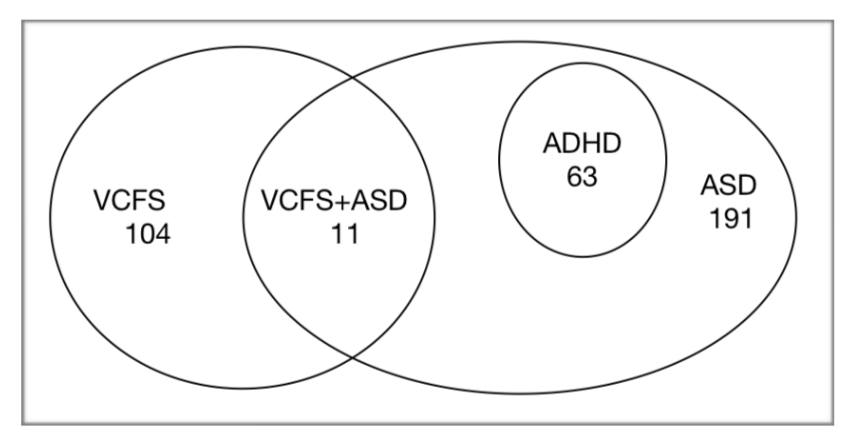
\includegraphics[width=0.6\textwidth]{Figures/Figure_3_1.png}}
  \caption{Venn Diagram of the division of diagnosis}
  \label{fig:Venn}
\end{figure}

However, not all children have taken all three parent-oriented review, figure \ref{fig:Reviews} gives details of how many children among the 369 have taken each of the tests. It can be observed that there only 48\% of subjects who have taken the VINE while majority have taken the ADI and the BASC.

\begin{figure}
\centering
  {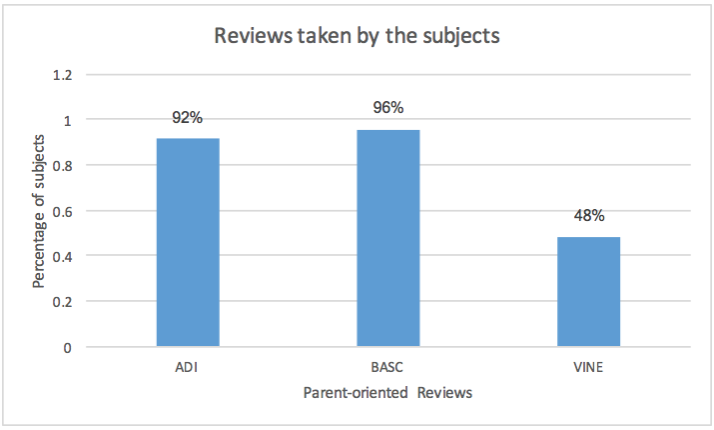
\includegraphics[width=0.6\textwidth]{Figures/Figure_3_2.png}}
  \caption{Reviews taken by subjects in percentage}
  \label{fig:Reviews}
\end{figure}
The verbal IQ, non-verbal IQ and full scale IQ of the subjects is measured, and the range of IQ is from 40 to 160 with a mean IQ of 100. Out of the 369 children, there are 252 male children which constitutes 68\% of the data and there are 117 female children which constitutes the rest 31\% of the data. The figure \ref{fig:Reviews2} gives information on how many children have taken the reviews based on gender. If our models were to be trained on this data, then it could be observed that models would be biased towards males over females as they are more dominant the dataset. On the male subjects, the classifier had an accuracy of 96.03\%, ROC Area value of 0.997 and F-measure of 0.959. On the other hand, the classifier gave an accuracy of 88.03\%, ROC Area value of 0.972 and F-measure of 0.851. Therefore, most of our models predict the diagnosis labels in the subgroup data for male subjects with a better accuracy of 7\% when compared to female subjects.
\begin{figure}
\centering
  {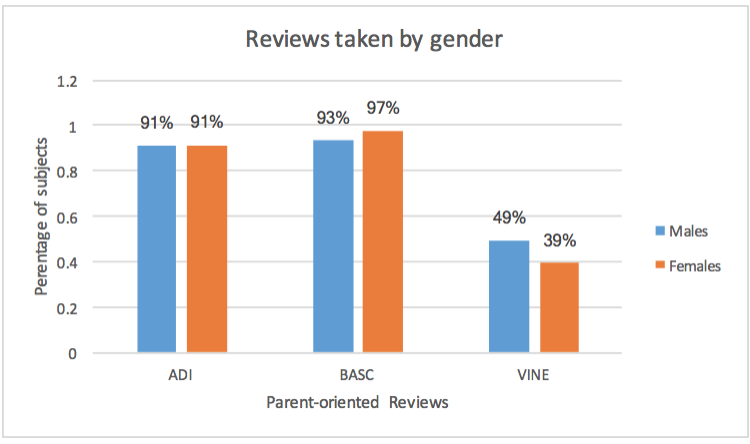
\includegraphics[width=0.6\textwidth]{Figures/Figure_3_3.png}}
  \caption{ Parent-oriented reviews taken by gender}
  \label{fig:Reviews2}
\end{figure}

Also, further analysis of the actual data shows that for certain subjects, certain feature values are missing. When the person has taken a parent-oriented review, then certain questions in the review were missing. So, features of each parent-oriented having missing values have been analyzed. It could be observed that, from subjects who have taken the VINE parent-oriented review, none of the feature values were missing. The features of ADI parent-oriented review and BASC parent-oriented review which had missing values are shown in figures\ref{fig:ADI} and \ref{fig:BASC} respectively. When considering the missing features for ADI, the missing sections have been considered as the parents have failed to fill a particular section of the review. Even though the missing values of individual sections is as high as 45\%, it can be seen that the missing values of each of the four domains is very low(A-2\%, BV-4\%, BNV-8\%, C-13\%, D-3\%). This shows that particular sub sections of the review are not filled, but overall sections in the review are filled. So, in the case of ADI, the missing features when handled accurately can avoid model over-fitting due to outliers. When we analyze the features of BASC, it was observed that only 4 out of 16 features had missing values. The feature `Adaptability' had 20\% of its features missing and the other features had very low percentage of missing values.
\begin{figure}
\centering
  {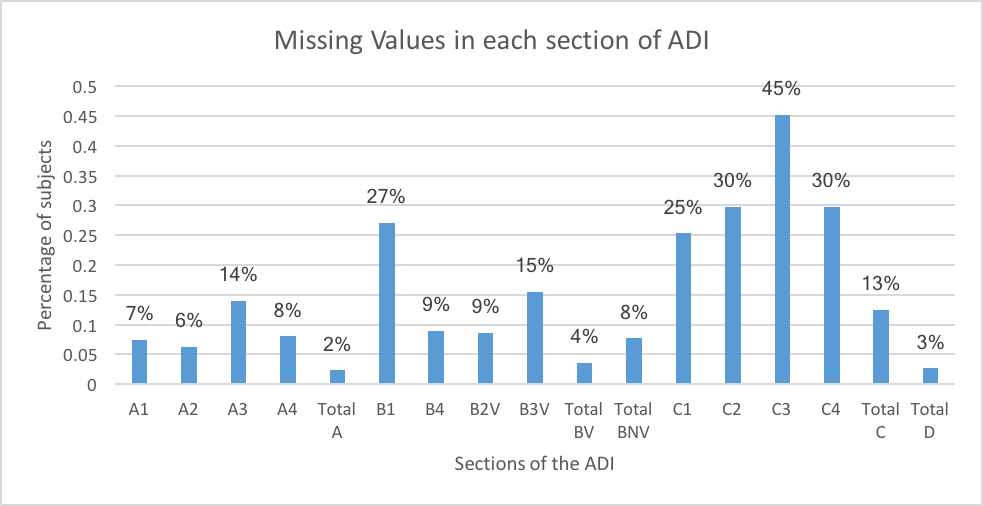
\includegraphics[width=0.6\textwidth]{Figures/Figure_3_4.png}}
  \caption{Analyzing missing values of features in ADI}
  \label{fig:ADI}
\end{figure}
\begin{figure}
\centering
  {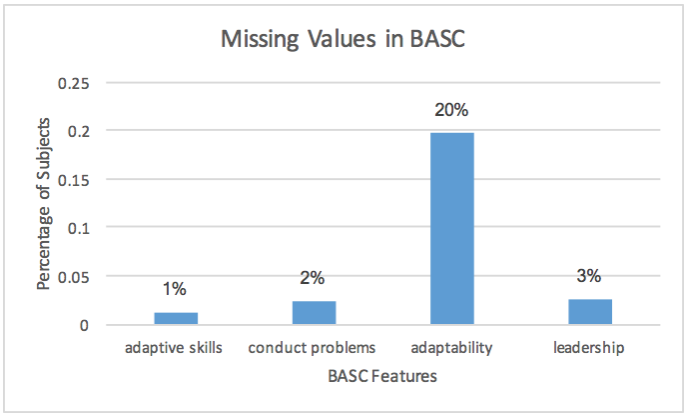
\includegraphics[width=0.6\textwidth]{Figures/Figure_3_5.png}}
  \caption{Analyzing missing values of features in BASC}
  \label{fig:BASC}
\end{figure}
\newline
In our research, when analyzing about the comorbid disorders ASD and ADHD, the `ABIDE' and `ADHD-200' datasets have also been used along with our actual dataset. These datasets have phenotypes and f(MRI) images of the brain and for our research the phenotypes aspect of the dataset has been taken. When analyzing how IQ is effecting the comorbidity of ASD and ADHD, the subjects from these datasets who have been diagnosed with ASD and ADHD were added to our dataset. The main reason behind this is that our dataset doesn’t contain any children with only ADHD. To keep our data balanced subjects were selected randomly from 539 ASD individuals and 285 ADHD individuals.
\section{Data Preprocessing}
This is one of the most important steps of the data mining process. The presence of noisy, irrelevant and unreliable data makes it difficult for knowledge discovery during the training phase of machine learning. Some of the preprocessing steps applied to our data to make it suitable for our training phase are as follows: 
\begin{itemize}
	\item Data Transformation- This is the process of converting the given data into a desired format. The most common transformation technique applied to our dataset is the conversion of  categorical features. Most of the data transformation steps that have been applied are given below and these steps are necessary for using the machine learning algorithms from sklearn package:
	\begin{compactenum}
		\item The feature `Sex' is converted to 1 (indicates male) and 0 (indicates female).
		\item All other feature columns whose attribute values are ‘YES/NO’ will be converted to 1  (for yes) and 0 (for no) .
		\item The target column `Diagnosis' is mapped to labels as follows: \begin{compactenum}\item ASD is 0 
\item ADHD+ASD is 1 
\item VCFS+ASD is 2 
\item VCFS is 3  \end{compactenum}
Also, when individual developmental disorders are studied or when we study comorbidity, the target column will be changed according. For example when analyzing ASD, all the children diagnosed with ASD will be mapped to 1 and others will be mapped to 0. Similar mapping will be done during different parts of our research.
	\end{compactenum}
Some parts of our research use machine learning algorithms from WEKA, for this purpose, the transformation technique used is to convert the data types of ADI features from numeric to nominal. Therefore, by applying these transformation techniques the data types will be correctly interpreted by the machine learning algorithms that will be used for our analysis.
\item Data Reduction- This is the process of reducing the given data to include only the necessary columns. Our data consists of many unique identifiers and unnecessary columns. By doing this, over-fitting of the data during the training phrase can be avoided. Over-fitting of our model means that our model is too closely fit to the data and it makes the model more complex than necessary.  The following are the steps taken to reduce our feature set:
	\begin{compactenum}
    \item The columns- `Subject ID', `Lab', `BASC', `VINE', `ADI' and `ADIAUTISM' are removed from the dataset and are not used by the model for prediction. The feature `ADIAUTISM' is a direct indicator of whether a child has ASD or not, hence it needs to be removed from our data. Now, the total number of features/variables on which the model will be trained is 92. 
	\item Further more, the columns which have totals for the ADI test have also been removed from the dataset, as these columns contain redundant feature information and are just simply sum of previous features. 
	\item Also, the age attribute has been condensed from four, that is three columns `ADI Age`, `BASC Age` and `VINE Age` remain. For the children who don’t have these age, their actual age from the `Age(Years)` is considered to be the age when the reviews were taken by the children. 
    \end{compactenum}
After applying the data reduction techniques on our data, the final number of features on which the training will be done is 73 including the target column `Diagnosis'. In WEKA, this step can be carried out using the Remove attribute feature. Hence, with the help of this step, our models will be able to generalize over our data.
\item Data Cleaning- It is a process of detecting, correcting or removing inaccurate instances from our data. The most important task in our data cleaning step is handling missing values. As seen in the data exploration section, most of our features have missing values. While handling missing values in our data, the structure of our data should not be effected, that is they should not become noise or outliers of our data. Hence, it is important that each features of our feature set are handled differently so that the structure of our actual data is maintained. The following are the steps as to how the missing values are handled:
\begin{compactenum}
\item Handling missing values for IQ test features- The PRI, VCI and FSIQ column’s missing values are replaced with the mean value which is 100. This has not affected the mean value of the dataset, so it is a good idea to replace missing values with 100. 
\item Handling missing values for ADI parent-oriented review features- The scores for ADI features/variables ranges from 0 to 2. In this case, the missing values are replaced with a 0 because this indicates not present. When the value is missing it is safe to assume that that the symptom is not present in the children than making any other assumptions and leading to false outcomes. 
\item Handling missing values for BASC parent-oriented review features- The scores have a mean of 50 and the standard deviation of 10. When the values are 70 it means it is critical. So, for this test the values are going to be replaced with the mean that is 50. For any value below 50, the score is not to be considered, hence, the missing values in the dataset are replaced with 50. 
\item Handling missing values for VINE parent-oriented review features- The scores are standard and the missing values are going to be replaced with 0. This is because most subjects don't have the VINE gets scores and the subjects that have taken the VINE tests have the results without any missing values. 
\end{compactenum}
\end{itemize}
After the preprocessing of the data, the model is trained on the modified features. The next sections discuss the training steps and the results obtained after training the model. Also, before training the model out of the 73 features, the features best used to train the model are selected so that the model can be trained correctly with these important features.

\section{Feature Selection}
Feature selection also known as variable selection is the process of selecting a subset of features from our given data. The different feature selection algorithms used in our research are LASSO regression\nomenclature{LASSO}{Least Absolute Shrinkage and Selection Operator}, ReliefF and Recursive Feature Elimination
\nomenclature{RFE}{Recursive Feature Elimination}. The LASSO regression method that selects subset of variable when there is highly correlated predictors in the data, as in our dataset.  On the other hand, ReliefF is a noise tolerant and robust algorithm which is independent of variable dependencies. While RFE uses an elimination process to select a subset of features recursively from our data. One or all of these feature selection algorithm have been applied on different aspects of our research and the results obtained are discussed in the following sections.

\subsection{Subgroup Diagnosis}
As part of our research, initially, predictions are done on the actual data sample. Feature selection algorithms are used on the preprocessed data which has 73 features and the best 5 features are selected. The root mean squared error \nomenclature{RMSE}{Root Mean Square Error} is used to analyze the performance of our feature selection models. Also, the best features are selected by doing 10-fold cross validation, that is at each fold the best features are taken and then finally best 5 features are found using a weighted average. ReliefF algorithm was not applied to our data to select best features as there are multi class labels in our data and ReliefF works well for binary classifiers. The RMSE for LASSO and RFE is 0.6837 and 0.66575. Both of these models have similar RMSE and hence, it can be said that these models are have similar performance measures when selecting the best features. However, LASSO has selected features from BASC and VINE, whereas RFE has selected features from ADI and are shown in table \ref{table:Subgroup}. So, there are no convergent features selected by these two algorithms.
%%table 3.1
\begin{table}[h]
\begin{center}
\begin{tabular}{|p{7 cm}|p{8 cm}|}
\hline
\textbf{LASSO} & \textbf{Recursive Feature Elimination}\\
\hline \hline
\begin{enumerate}
\item Performance IQ
\item Activities of Daily Living
\item Vineland daily living
\item Adaptability
\item Vineland Composite 
\end{enumerate}  & \begin{enumerate}
\item Criteria for repetitive behaviors and stereotyped patterns
\item Criteria for qualitative impairments in reciprocal social interaction
\item Quality of social overtures
\item Offers comfort
\item Inappropriate questions or statements
\end{enumerate} \\
\hline
\end{tabular}
\end{center}
\caption{Best 5 variables by different feature selection algorithm for Subgroup Diagnosis}
\label{table:Subgroup}
\end{table}

\subsection{Comorbid Developmental Disorders}
There are two groups of comorbid disorders that are analyzed in our research. The first one is ASD and ADHD comorbidity and the other group is ASD and VCFS comorbidity. The actual data is divided to separate ASD and ASD+ADHD to analyze the comorbid disorders ASD and ADHD. This data consists of 254 subjects who have been diagnosed with ASD, out of which 63 subjects have ADHD as well. This data consists of 190 males and 64 females where 53 males  and 10 females have ADHD along with ASD. For analyzing ASD and VCFS comorbidity, the data used consists of 115 subjects diagnosed with VCFS and 11 have ASD as well. Even though there are 49 females and 55 males, this data is more balanced than other data that we have used so far. The best features for both these comorbidities is analyzed in this section. 
%table 3.2
\begin{table}[h]
\begin{center}
\begin{tabular}{|p{5 cm}|p{5 cm}|p{6 cm}|}
\hline
\textbf{ReliefF} & \textbf{LASSO} & \textbf{Recursive Feature \newline Elimination}\\
\hline \hline
\begin{enumerate}
\item Vineland socialization
\item Attention problems
\item Performance IQ
\item Vineland\newline Communication
\item Vineland Composite
\end{enumerate}  & \begin{enumerate}
\item Vineland socialization
\item Quality of \newline social overtures
\item Offering to share
\item Inappropriate questions or statements
\item Attention problems
\end{enumerate} & \begin{enumerate}
\item Quality of social overtures
\item Inappropriate questions or statements
\item Abnormality of development evident at or before 36 months
\item Criteria for Qualitative impairments in reciprocal\newline social interaction
\item Conventional/Instrumental Gestures
\end{enumerate} \\
\hline
\end{tabular}
\end{center}
\caption{Best 5 variables by different feature selection algorithm for ASD and ADHD comorbidity}
\label{table:comorbidASD}
\end{table}

For ASD and ADHD comorbid disorders, the best 5 features from the three feature selection algorithms are given in table \ref{table:comorbidASD}. The RMSE for LASSO, ReliefF and RFE is 0.289, 0.493 and 0.224 respectively. So, it shows that RFE and LASSO are performing better than ReliefF feature selection algorithm as they have lower RSME values. The LASSO feature selection algorithm has selected features from all three parent-oriented reviews and the RFE feature selection algorithm as selected all variables from ADI review. While the ReliefF has selected variables from BASC and VINE. It can be seen that there are convergent variables in the LASSO feature selection algorithm.

The best features for ASD and VCFS comorbidity selected when applying the three feature selection algorithms is given in table \ref{table:comorbidVCFS}. The RMSE for LASSO, ReleifF and RFE is 0.0093, 0.9484 and 0.07 respectively. By the observed RMSE values, it can be observed that LASSO and RFE high performance and ReliefF has poor performance. another observation made after looking at the features is that there no convergent features from different parent-oriented reviews. In fact, the LASSO selects the features from BASC, ReliefF from VINE and RFE from ADI. The only convergent feature is the `Performance IQ' selected by both LASSO and ReliefF.
%Table 3.3
\begin{table}[h]
\begin{center}
\begin{tabular}{|p{5 cm}|p{5 cm}|p{6 cm}|}
\hline
\textbf{LASSO} &\textbf{ReliefF} & \textbf{Recursive Feature \newline Elimination}\\
\hline \hline
\begin{enumerate}
\item Anxiety
\item Hyperactivity
\item Performance IQ
\item Conduct Problems
\item Depression
\end{enumerate}  & \begin{enumerate}
\item Verbal IQ
\item Vineland Composite
\item Performance IQ
\item Full Scale IQ
\item Vineland Daily Living
\end{enumerate} & \begin{enumerate}
\item Criteria for Repetitive behaviors and stereotyped \newline patterns
\item Repetitive use of objects or interest in parts of objects
\item Verbal Rituals
\item Criteria for Communication
\item Hand and Finger\newline mannerisms
\end{enumerate} \\
\hline
\end{tabular}
\end{center}
\caption{Best 5 variables by different feature selection algorithm for ASD and VCFS comorbidity}
\label{table:comorbidVCFS}
\end{table}

\subsection{Individual Developmental Disorders Diagnosis}
Our data consists of information related to three different developmental disorders that is ASD, VCFS and ADHD. For each of these disorders, the features are analyzed and the best features are found. The target label `Diagnosis' is converted to `ASD Diagnosis', `ADHD Diagnosis' and `VCFS diagnosis' for each of the disorders. Then, the 73 features preprocessed data is given as input to our feature selection algorithms and the best features for each developmental disorder are observed.
%Table 3.4-
\begin{table}[h]
\begin{center}
\begin{tabular}{|p{5 cm}|p{5 cm}|p{6 cm}|}
\hline
\textbf{LASSO} &\textbf{ReliefF} & \textbf{Recursive Feature \newline Elimination}\\
\hline \hline
\begin{enumerate}
\item Behavioral Symptoms
\item Performance IQ
\item Full Scale IQ
\item Adaptive Skills
\item Externalizing \newline problems
\end{enumerate}  & \begin{enumerate}
\item Activities of Daily\newline Living
\item Vineland \newline Communication
\item Vineland Composite
\item Vineland Daily Living
\item Functional \newline Communication 
\end{enumerate} & \begin{enumerate}
\item Criteria for Repetitive behaviors and stereotyped\newline patterns
\item Use of other's body to \newline communicate
\item Criteria for Qualitative impairments in reciprocal social interaction
\item Hand and Finger \newline mannerisms
\item Repetitive use of objects or interest in parts of \newline objects
\end{enumerate} \\
\hline
\end{tabular}
\end{center}
\caption{Best 5 variables by different feature selection algorithm for ASD}
\label{table:ASD}
\end{table}

The best features for distinguishing children with ASD from those who don't have it are given in table \ref{table:ASD}. The RMSE values for LASSO, RFE and ReliefF are 0.181, 0.218 and 0.523. This shows that LASSO and RFE are performing better than ReliefF due to the low RSME scores. LASSO selects the best features from the BASC parent-oriented review, ReliefF selects from both the BASC and the VINE parent-oriented review and RFE selects from ADI. Also, it can be observed that there is no overlap of features by all three feature selection algorithms.

%Table 3.5
\begin{table}[t]
\begin{center}
\begin{tabular}{|p{5 cm}|p{5 cm}|p{6 cm}|}
\hline
\textbf{LASSO} &\textbf{ReliefF} & \textbf{Recursive Feature \newline Elimination}\\
\hline \hline
\begin{enumerate}
\item Performance IQ
\item Full Scale IQ
\item Behavioral Symptoms
\item Adaptive Skills
\item Direct Gaze
\end{enumerate}  & \begin{enumerate}
\item Performance IQ
\item Vineland socialization
\item Vineland \newline communication
\item Vineland daily living
\item Vineland composite
\end{enumerate} & \begin{enumerate}
\item Inappropriate questions or statements
\item Quality of social overtures
\item Conventional/Instrumental Gestures
\item Criteria for Qualitative impairments in reciprocal\newline social interaction
\item Offers comfort
\end{enumerate} \\
\hline
\end{tabular}
\end{center}
\caption{Best 5 variables by different feature selection algorithm for ADHD}
\label{table:ADHD}
\end{table}

%Table 3.6
\begin{table}[t]
\begin{center}
\begin{tabular}{|p{5 cm}|p{5 cm}|p{6 cm}|}
\hline
\textbf{LASSO} &\textbf{ReliefF} & \textbf{Recursive Feature\newline Elimination}\\
\hline \hline
\begin{enumerate}
\item Hyperactivity
\item Criteria for Qualitative impairments in \newline reciprocal social interaction
\item Pronominal reversal
\item Vineland \newline Communication
\item Vineland Socialization
\end{enumerate}  & \begin{enumerate}
\item Activities of Daily Living
\item Functional \newline Communication 
\item Vineland \newline Communication
\item Vineland daily living
\item Vineland composite
\end{enumerate} & \begin{enumerate}
\item Criteria for Repetitive behaviors and stereotyped\newline patterns
\item Use of other's body to \newline communicate
\item Pronominal reversal
\item Neologisms/idiosyncratic language
\item Stereotyped Utterances \& delayed echolalia
\end{enumerate} \\
\hline
\end{tabular}
\end{center}
\caption{Best 5 variables by different feature selection algorithm for VCFS}
\label{table:VCFS}
\end{table}
The children with ADHD and those who don't have can be distinguished using the best features given in table \ref{table:ADHD}. The RMSE values for LASSO, RFE and ReliefF are 0.190, 0.201 and 0.407. The LASSO selects features from BASC, while the ReleifF selects from VINE and RFE selects from ADI. Even in this case there are no convergent parent-oriented reviews features except the Performance IQ feature. As the RMSE values are low for LASSO and RFE, the models are performing better than ReliefF.

For the developmental disorder VCFS, the RMSE values for LASSO, RFE and ReliefF are 0.189, 0.308 and 0.555. The best features selected by each of the three feature selection algorithms are given in table \ref{table:VCFS}. LASSO select features from all of the three parent-oriented reviews, while ReliefF selects from BASC and VINE. On the other hand, RFE selects from ADI. In this case, the convergent features are from ADI and VINE which are selected by LASSO.

When all of the feature selection algorithms are compared, it can be seen that RFE usually tends to select algorithms from the ADI parent-oriented review, while ReleifF selects mostly from VINE parent-oriented review and sometimes from BASC. LASSO is the only feature selection algorithm that has selected features from all three parent-oriented reviews. LASSO and RFE are both performing better than ReliefF. However, LASSO feature selection algorithm can be considered to be doing a better job as it has selected features from all three reviews. Also, LASSO assigns coefficients to each of the features and these coefficients can be negative or positive. It eliminates all the unimportant features by assigning them weights 0. Therefore, for most parts of our research only LASSO features have been used for our analysis.

\chapter{Investigating the Subgroup Diagnosis} \label{ch:meas}
\thispagestyle{plainbottom}
The dataset collected in different labs consists of different groups of diagnosis. Each of these diagnosis is dependent on the features of the reviews. In this chapter, analysis of these groups has been done using different Machine Learning techniques. For the purpose of understanding the diagnosis, initially unsupervised learning technique (k-means clustering) is applied. Then, feature selection algorithms are applied to understand the feature importance of our entire data available. Finally, supervised learning techniques have been applied to predict each of these different groups diagnosis. Also, the features of the data are divided into four sections (IQ, ADI, BASC, VINE) and supervised learning techniques have been applied to predict the diagnostic label using each section of features.

\section{Unsupervised Learning Techniques to Categorize Subjects}
The dataset is clustered using $K$-Means Clustering algorithm to analyze the clusters in the dataset. The dataset consists of 73 features/variables after the preprocessing of our data. For applying $K$-Means clustering, the dimension of the data has to be reduced further and for this purpose Principal Component Analysis\nomenclature{PCA}{Principal Component Analysis} has been used. The PCA transforms the set of features of the dataset orthogonally. Also, PCA handles the missing values and the outliers in our data, so for this section of our analysis missing values have not be handled as part of preprocessing. For the given dataset, the PCA algorithm in sklearn package in python is used. For visualizing our dataset, the PCA algorithm is applied to find the first two principle components of our dataset, so that our data can be visualized in 2D. After performing PCA, the figure \ref{fig:41} gives the visualization of our dataset. From this figure, it can be seen that there are four different/unique groups. However, there is an overlap between 2 groups as children diagnosed with `ASD+ADHD` and falling into the group of children diagnosed with `ASD`. Similarly, children diagnosed with `VCFS+ASD` fall into the group of children diagnosed with `VCFS`. Due to this overlap there are only two distinguishable majority groups in our subgroup data.
\begin{figure}
\centering
  {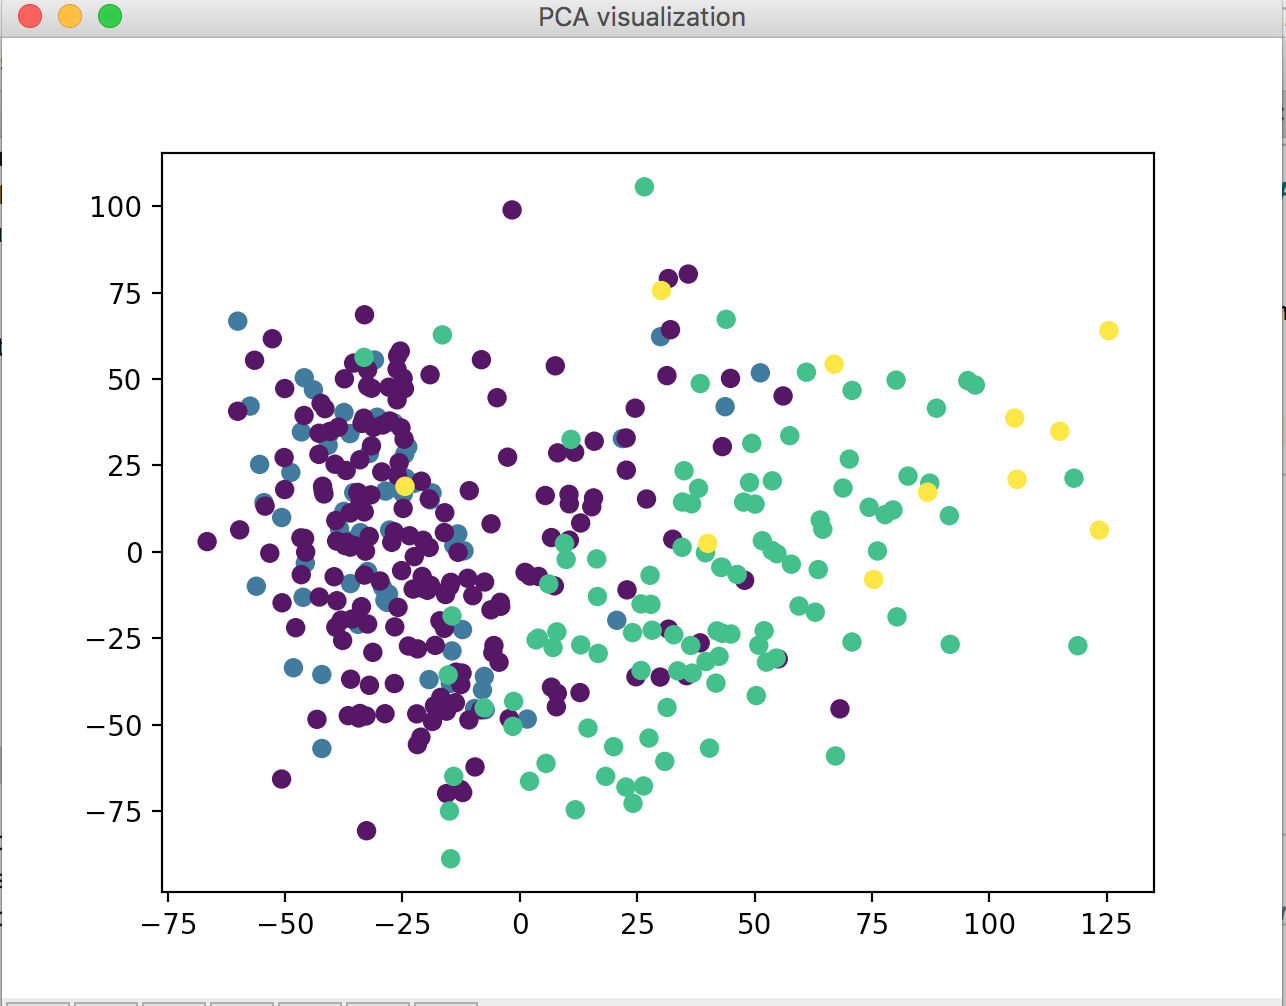
\includegraphics[width=0.6\textwidth]{Figures/Figure_4_1.png}}
  \caption{Analyzing missing values of features in BASC}
  \label{fig:41}
\end{figure}
Now, on this reduced data from PCA has been given as input to K-Means clustering algorithm without the diagnostic labels. The $K$-Means clustering algorithm available in sklearn package has been used. As proper analysis of the data needs to be done, the $k$ value was varied from 2 to 5. Since, there are 4 different diagnostic groups in our dataset, the data has been cluster unto $k$ value equal to 5. The main reason behind this is to check if there are any pure clusters. For each of these $k$ values, the visualization is given in the figure \ref{fig:42}.

In the figure \ref{fig:42}, when $k$ is equal to 2, cluster 1 (yellow color) consists of  all VCFS diagnosed children (including children with VCFS+ASD) and cluster 2(purple color) has ASD and ASD+ADHD diagnostic children. However, there are 16 children in cluster 1 who have ASD only and 1 child in cluster 1 having ASD+ADHD. Then, the cluster size was increased to 3 and it was observed that cluster 1 consisted of all the VCFS+ASD children. Further analysis showed that children with ASD and ASD+ADHD were spread over all the three clusters, whereas children with VCFS only were spread over first two clusters. When the cluster size was increased further to 4 and 5, it was observed that the clusters where more of a mixture, there was no purity in the clusters. The main reason for this could be that there are lot of features overlap for each of the diagnostics.
\begin{figure}
\centering
  {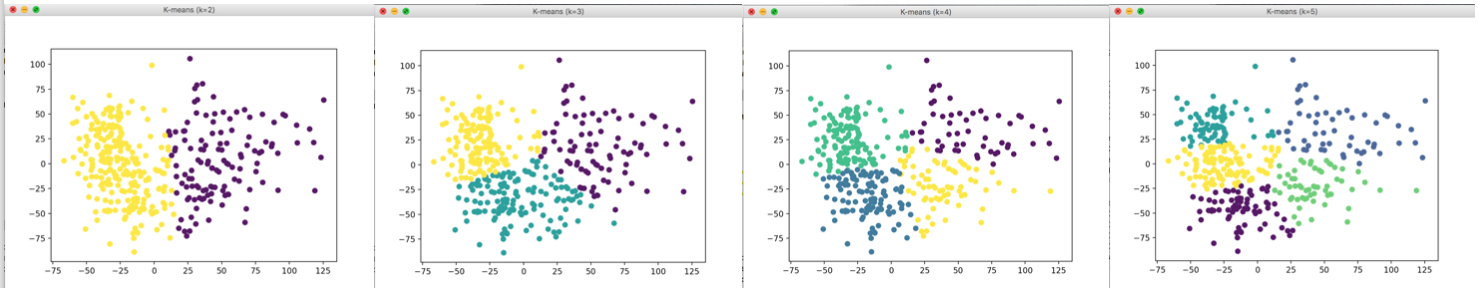
\includegraphics[width=0.9\textwidth]{Figures/Figure_4_2.png}}
  \caption{After applying $k$-means clustering on the PCA reduced dataset}
  \label{fig:42}
\end{figure}
% * <reza@data.syr.edu> 2018-04-12T18:02:07.357Z:
%
% ^.

As mentioned above, PCA handles missing values, if the preprocessed data were given as input to the K-Means then the accuracy of the K-Means clustering algorithm dropped to 83.5\%, that means that there was more randomness in the data and higher chances of not grouping them accurately. However, the average accuracy of clustering the data was 95.3\%. After, K-means clustering it could be said that children diagnosed with VCFS are closely clustered that is they belonged to one cluster most of the times and more specifically children with VCFS+ASD were most likely to be in the same cluster than the other diagnostic subgroups.

\section{Supervised Learning Techniques to Predict Diagnostic Groups}
The subgroup dataset after preprocessing is trained using different supervised learning techniques. As the dataset is small and simple, there is no need for very complex classification models. The data is loaded into WEKA and different classification algorithms have been applied on this data. The algorithms are compared based on different metrics as seen in table \ref{table:41}. The different metrics on which the models are evaluated are Accuracy, Precision, Recall, ROC Area and F-measure. Cross validation technique has been applied on the data and the dataset has been divided into 10 folds wherein training is done on 9 folds and testing on one. The different classification algorithms that have been used to train our models are Naive Bayes, Logistic Regression, Multi-class classifier and Random Forest. Since, our dataset consists of feature relations and multiple class labels, the above algorithms were chosen.
%table 4.1
\begin{table}[h]
\begin{center}
\begin{tabular}{|l|c|c|c|c|c|}
\hline
\textbf{ML Algorithm} & \textbf{Precision}&	\textbf{Recall}&	\textbf{F-measure}&	\textbf{ROC Area}&	\textbf{Accuracy}\\
\hline \hline
Naive Bayes & 0.934 &	0.924 &	0.928 &	0.981& 	92.4119\%\\
\hline
Logistic Regression &	0.926&	0.924&	0.924&	0.990&	92.4119\%\\
\hline
Multi Class Classifier&	0.902&	0.902&	0.902&	0.980&	90.2439\%\\
\hline
Random Forest&	0.960	&0.959	&0.957	&0.994&	94.85\%\\
\hline
\end{tabular}
\end{center}
\caption{Supervised learning techniques to predict subgroup diagnosis}
\label{table:41}
\end{table}

Among the different supervised learning techniques applied on the dataset, Random Forest has a better accuracy and ROC Area value.\nomenclature{ROC}{Receiver Operator Characteristic} So, it can be said that Random Forest is doing a good job of classifying our dataset. Also, each of the class labels are measured to check their precision and recall. For the group of children diagnosed with ASD+ADHD, precision and recall of Random Forest is 96.6\% and 90.5\% respectively. Similarly the precision and recall for the children diagnosed with ASD is 93.9\% and 96.3\% respectively. For the children diagnosed with VCFS, precision and recall are 95.4\% and 100\% respectively. However, precision and recall for the children with VCFS+ASD is 100\% and 45\% respectively and this could be because their are a low percentage of children with VCFS+ASD when compared to the other diagnostic groups.   Now, rather than giving the entire feature set, only the best features selected from the three different feature selection algorithms as in chapter 3 are given to machine learning algorithms to predict our subgroup diagnosis. The results of each of the feature selection algorithms are given below in table \ref{table:42} by LASSO and table \ref{table:43} by RFE.
%table 4.2
\begin{table}[h]
\begin{center}
\begin{tabular}{|l|c|c|c|c|}
\hline
\textbf{ML Algorithm} & \textbf{Accuracy}&	\textbf{Precision}&	\textbf{Recall}&	\textbf{ROC Area}\\
\hline \hline
Naive Bayes&	66\%	&0.690&	0.656&	0.851\\
\hline
Logistic Regression&	73\%&	0.605&	0.732&	0.827\\
\hline
Multi Class Classifier&	72.6\%	&0.584	&0.7267&	0.829\%\\
\hline
Random Forest&	70.4\%&	0.680&	0.705	&0.859\%\\
\hline
\end{tabular}
\end{center}
\caption{Supervised learning techniques to predict subgroup diagnosis by LASSO}
\label{table:42}
\end{table}

%table 4.3
\begin{table}[h]
\begin{center}
\begin{tabular}{|l|c|c|c|c|}
\hline
\textbf{ML Algorithm} & \textbf{Accuracy}&	\textbf{Precision}&	\textbf{Recall}&	\textbf{ROC Area}\\
\hline \hline
Naive Bayes&	83.1\%	&0.836&	0.832&	0.924\\
\hline
Logistic Regression&84.2\%&	0.842&	0.843&	0.917\\
\hline
Multi Class Classifier&	84.2\%&	0.841&	0.843&	0.916\\
\hline
Random Forest&84.5\%&	0.840&	0.846&	0.912\\
\hline
\end{tabular}
\end{center}
\caption{Supervised learning techniques to predict subgroup diagnosis by RFE }
\label{table:43}
\end{table}
From the tables \ref{table:42} and \ref{table:43}, the features selected from the RFE feature selection are preforming better than out LASSO feature selection algorithm. However, when using only the best 5 features, the accuracy of the random forest drops from 96\% to 84\% but the ROC Area value is still high in the case of Random forest. Also, with the help of LASSO features we selected all the relevant features with non-zero weights. Out of the 73 features after preprocessing, the relevant features were 45 and when Random forest model was trained on these 45 features, an accuracy of 92\% was achieved. 
\begin{figure}
\centering
{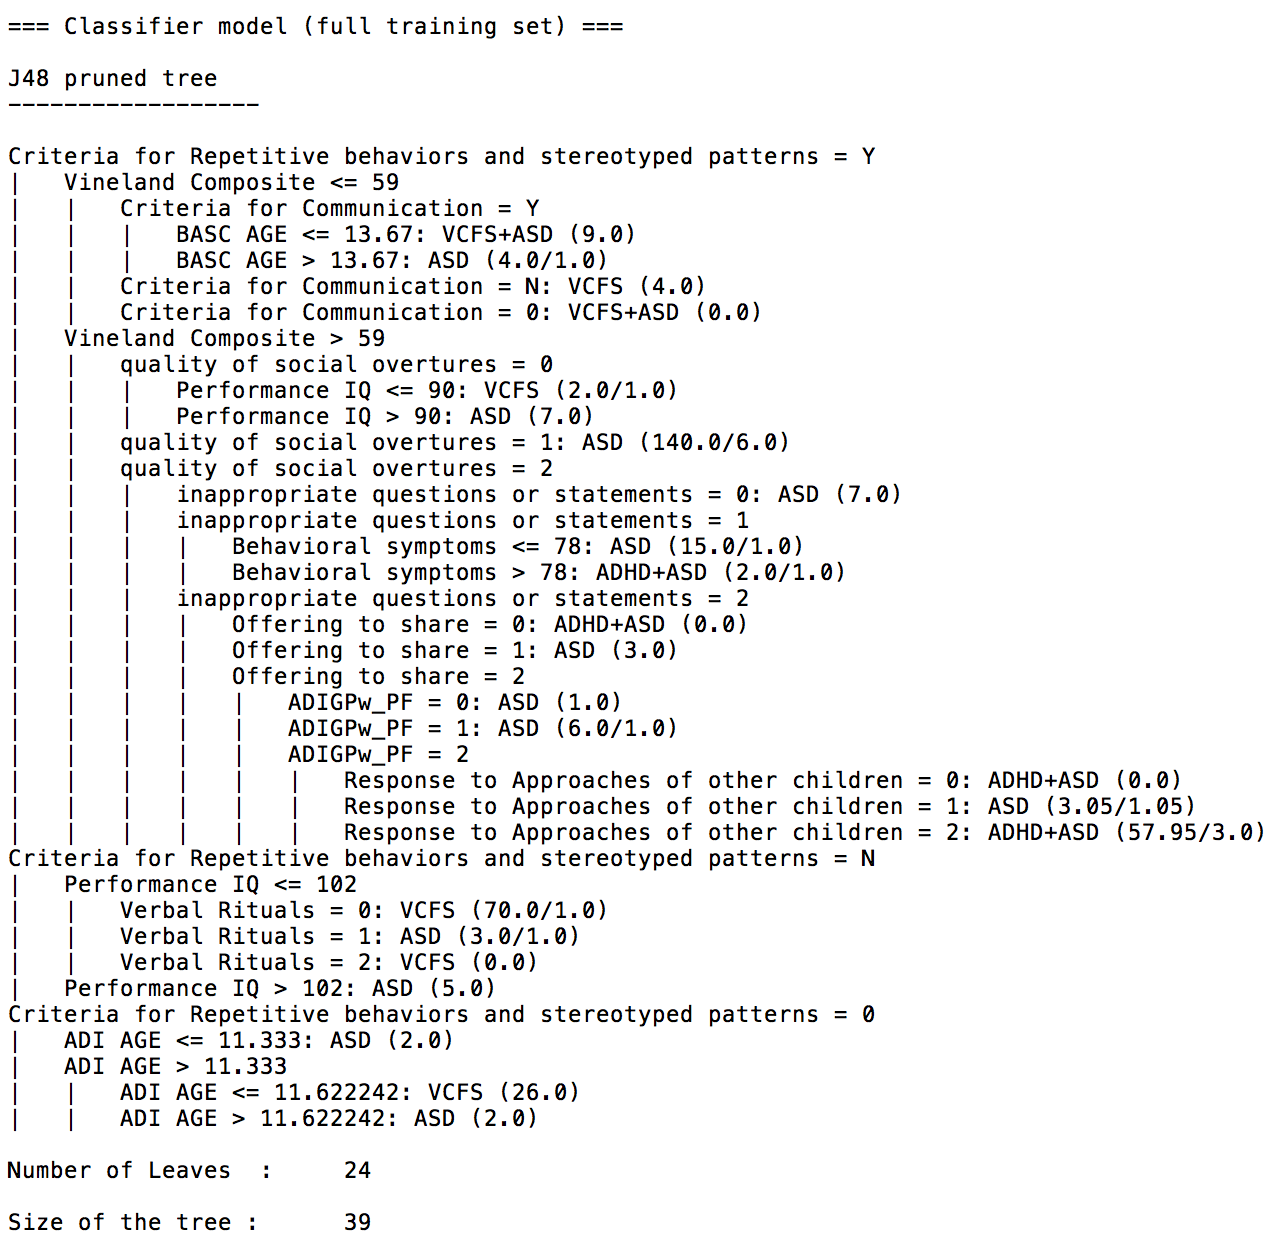
\includegraphics[width=0.5\textwidth]{Figures/Figure_4_3.png}}
  \caption{J48 pruned tree}
  \label{fig:43}
\end{figure}

Since, Random Forest is doing a good job at predicting the subgroup features, another types of tree algorithm J48 also known as ID3 from WEKA is used to represent our model in the form of the tree. The figure \ref{fig:43} shows the results obtained from the J48 algorithm.It had an accuracy, precision and recall of 87\%. Also, precision and recall for the subgroups ASD, ASD+ADHD, VCFS ranges from 81\% to 90\%, however, the precision and recall for VCFS+ASD group is 60\%.

\subsection{Predicting Subgroup Diagnosis using the IQ feature set}
In this section of our research, IQ feature set consists of 3 features and using only these features, the subgroup diagnosis of the data is predicted. So, only these 3 features are given to our machine learning algorithms and the results are observed in table \ref{table:44}.
%table 4.4
\begin{table}[h]
\begin{center}
\begin{tabular}{|l|c|c|c|c|c|}
\hline
\textbf{ML Algorithm} &	\textbf{Precision}&	\textbf{Recall}&	\textbf{F-measure}& \textbf{ ROC Area}&	\textbf{Accuracy}\\
\hline \hline
Random Forest&	0.604&	0.623&	0.612&	0.802&	66.32\%\\
\hline
Naive Bayes&	0.401&	0.485&	0.438&	0.612&	48.50\%\\
\hline
Logistic Regression&	0.546&	0.580&	0.517&	0.716&	57.99\%\\
\hline
\end{tabular}
\end{center}
\caption{Supervised learning techniques to predict subgroup diagnosis by IQ feature set}
\label{table:44}
\end{table}

When all the different machine learning algorithms are compared, then Random forest is performing better than other machine learning algorithms. However, the Random forest has very low accuracy of 66\%. It has dropped from 92\% to 66\% which is very low and not an accurate model for the purpose of prediction. In this case, it could be mainly because the IQ range is similar for all the diagnostic groups.

\subsection{Predicting Diagnosis based on ADI feature set}
The ADI review has 45 features/variables in the dataset that analyze the behavior of children. These attributes are used to predict the diagnosis of the child. Initially, many supervised techniques have been applied on the Subgroup data and the various metrics of evaluation are listed in the table \ref{table:45}. 
%table 4.5
\begin{table}[h]
\begin{center}
\begin{tabular}{|l|c|c|c|c|c|}
\hline 
\textbf{Classifier} &	\textbf{Precision} &	\textbf{Recall} &	\textbf{F-measure} & \textbf{ROC Area}&	\textbf{Accuracy}\\
\hline \hline
Random Forest	&0.966&	0.965&	0.964&	0.976&	96.47\%\\
\hline
Naive Bayes&0.876	&0.870&	0.869&	0.959&	86.99\%\\
\hline
Logistic Regression&0.868&	0.864	&0.866&	0.936&	86.44\%\\
\hline
\end{tabular}
\end{center}
\caption{Supervised learning techniques to predict subgroup diagnosis by ADI feature set}
\label{table:45}
\end{table}

When using the reduced feature set from LASSO, which consisted of 45 features, these features were a combination of all the three parent-oriented reviews and the accuracy of our Random Forest model was 92\%. However, when we use only the 45 ADI features , the accuracy of our Random Forest model is 96\% with high precision and recall. Since, random forest model is doing great when predicting the subgroup diagnosis with ADI feature set, another similar algorithm J48 has been applied to our data. this will help our model to be concisely visualized in the form of a tree. The results of J48 in the form of a tree are given in figure \ref{fig:44}. The accuracy of our model is 87\%.

\begin{figure}
\centering
  {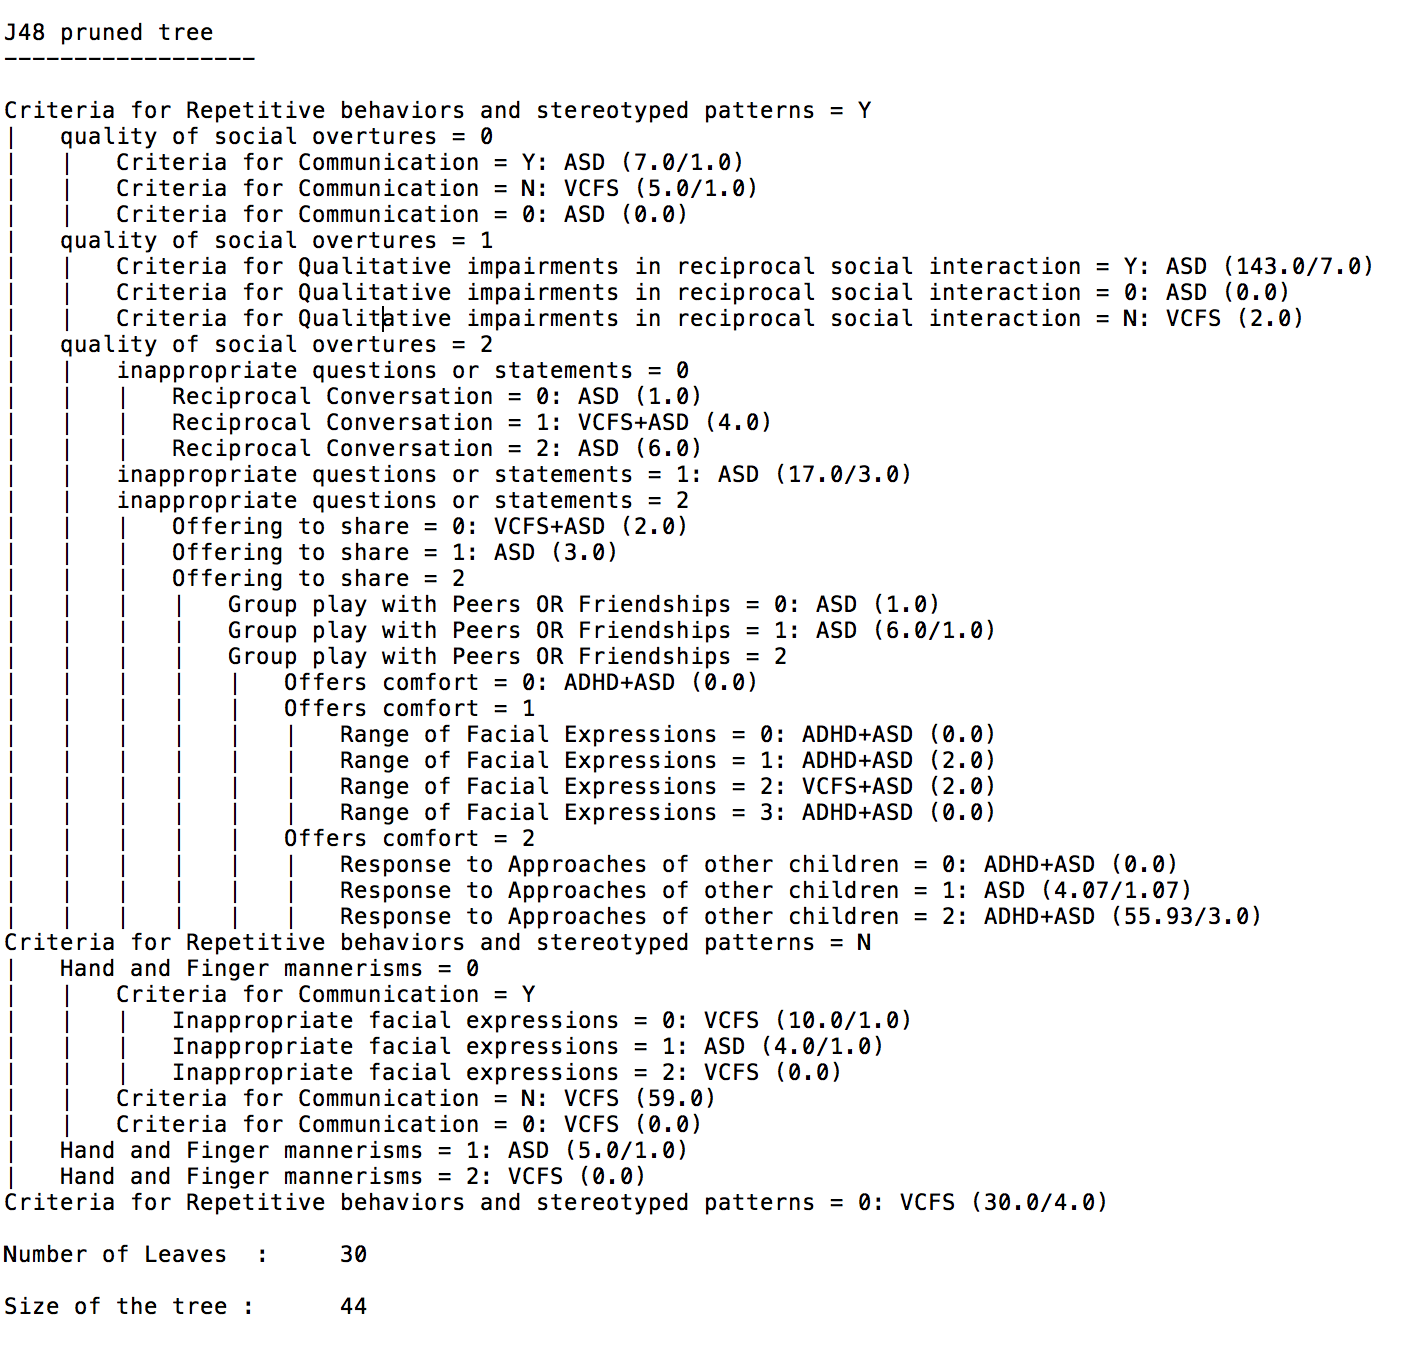
\includegraphics[width=0.6\textwidth]{Figures/Figure_4_4.png}}
  \caption{J48 pruned tree with ADI feature set}
  \label{fig:44}
\end{figure}

\subsection{Predicting Diagnosis based on BASC feature set}
BASC is another parent-oriented review where there are 19 different features to analyze the behaviors of the children. These features of BASC are used to predict the diagnosis of the child. Initially, many supervised techniques have been applied on the Subgroup data diagnosis and the various metrics of evaluation are listed in the table \ref{table:46}. 
%table 4.6
\begin{table}[h]
\begin{center}
\begin{tabular}{|l|c|c|c|c|c|}
\hline
\textbf{ML Algorithm} &	\textbf{Precision}&	\textbf{Recall}&	\textbf{F-measure}& \textbf{ROC Area}&	\textbf{Accuracy}\\
\hline \hline
Random Forest&0.713	&0.751&	0.712	&0.879&	75.06\%\\
\hline
Naive Bayes&0.694	&0.659&	0.671	&0.841&	65.85\%\\
\hline
Logistic Regression&0.693	&0.713	&0.694&	0.861&	71.27\%\\
\hline
\end{tabular}
\end{center}
\caption{Supervised learning techniques for subgroup diagnosis by BASC feature set}
\label{table:46}
\end{table}

Random Forest is performing better than all other machine learning algorithms with an accuracy of 75.06\%, but this accuracy is not high for predicting subgroup diagnosis as compared to previous models of predictions.

\subsection{Predicting Diagnosis based on VINE feature set}
VINE is also another parent questionnaire, when compared to other two reviews, VINE has fewer features for analyzing the behaviors. Also, the children who have taken the VINE tests are less compared to other two tests. These 4 features of VINE are used to predict the diagnosis of the child. Initially, many supervised techniques have been applied on the Subgroup data and the various metrics of evaluation are listed in the table \ref{table:47}. In the case of VINE parent-oriented review, the best model is by Logistic Regression with an accuracy of 71\% and the random forest only gives an accuracy of 68\%. 
%table 4.7
\begin{table}[h]
\begin{center}
\begin{tabular}{|l|c|c|c|c|c|}
\hline
\textbf{ML Algorithm} &	\textbf{Precision}&	\textbf{Recall}&	\textbf{F-measure}& \textbf{ROC Area}&	\textbf{Accuracy}\\
\hline \hline
Random Forest& 0.560&	0.680&	0.612&	0.785&	68.02\%\\
\hline
Naive Bayes& 0.550&	0.553&	0.517&	0.600&	55.28\%\\
\hline
Logistic Regression& 0.656&	0.710&	0.680&	0.787&	71\%\\
\hline
\end{tabular}
\end{center}
\caption{Supervised learning techniques for subgroup diagnosis by VINE feature set}
\label{table:47}
\end{table}

\section{Observations}
The machine learning algorithms applied to distinguish the subgroups are doing good job and the results are great. Among all the machine learning algorithms that have been applied on our actual data, Random Forest is doing well at predicting our subgroup diagnosis labels. This shows that  the model is successfully at finding the required relations between the feature set to the diagnostic labels. Using LASSO feature selection algorithm, the features were reduced from 72 to 45 and the performance of the Random Forest model is still very good. This shows that not all the 72 features are required to predict the diagnosis of the children with different combinations of these developmental disorders.

Apart from this when the feature set was divide into four different sub features set, it was observed that using the IQ features, the BASC parent-oriented review features and VINE parent-oriented review features can not be used individually to define models that can predict the subgroup diagnosis accurately. On the other hand, ADI parent-oriented reviews have resulted in good models when predicting the subgroup diagnosis features. The Random Forest model designed with ADI features is better than the Random Forest model built with 45 features from LASSO. Also, the J48 pruned tree with the entire feature set has similar model performance as the J48 pruned tree with only ADI parent-oriented reviews, that is both models have an accuracy of 87\%. When the ADI features are analyzed in more depth, it could be seen that some of the important features as selected by the J48 algorithm among the 45 ADI features are as follows:
\begin{compactenum}
\item Criteria for Repetitive behaviors and stereotyped patterns
\item Criteria for Qualitative impairments in reciprocal social interaction
\item Inappropriate questions and statements
\item Offers Comfort
\item Quality of social overtures
\item Offering Comfort
\item Range of Facial Expressions 
\item Hand and finger mannerisms
\item Response to approaches of other children
\item Reciprocal Conversation
\end{compactenum}

Most of the features that have been selected are key symptoms of the developmental diagnosis that our research is trying to predict in the children. This shows that our models are able to find valuable information like this from our features. As models built with ADI features are doing well and comparable with the entire feature set, it can be said that ADI features are sufficient. Therefore, ADI parent-oriented review is better than BASC and VINE parent-oriented review for building models to predict the subgroup diagnosis.
\chapter{Analyzing Comorbidity of Developmental Disorders }
The actual data is divided into two types, the first deals with children who are diagnosed with ASD and both ASD and ADHD and the second deals with children who are diagnosed with VCFS, ASD and both these disorders. In the first half go this chapter using the first data, the comorbid disorders ASD and ADHD are analyzed and then in the second half of this chapter comorbid disorders VCFS and ASD are analyzed. Different supervised and unsupervised machine learning techniques will be applied in both the sections to build models and results obtained will be analyzed. Also, analysis will be done on the features selected in chapter 3 by building models using these features and comparing them with other models. 
\section{ASD and ADHD Comorbidity}
The data being used to analyze ASD and ADHD comorbidity consists of 254 subjects who have been diagnosed with ASD, out of which 63 subjects have ADHD as well. This data consists of 190 males and 64 females where 53 males and 10 females have ADHD along with ASD. Initially, $K$-Means algorithm with PCA has been applied to check if these two groups could be distinguished by our $K$-means algorithm. However, our means algorithm was not able to distinguish these two groups of children in both two and three dimensions. There was an overlap in the feature values and our unsupervised learning technique couldn’t result in pure clusters even as we increased the size of $k$ to 9. So, supervised learning techniques were applied on the data and this is discussed in the next sub section.

\subsection{Supervised Learning Techniques to predict ADHD in Autistic children}
The data used for this analysis has already been preprocessed in the chapter 3, now this data is loaded into WEKA and different machine learning classifiers in WEKA are used to build our models. The different Machine Learning classifiers used for our analysis are Naive Bayes, Logistic Regression, Random Forest, Support Vector Machines and K-Nearest Neighbors. These algorithms have been applied to our data to build models as they are suitable for data and these algorithms work well with the type of data that we have. The results obtained from our machine learning algorithms on our data is given below in table \ref{table:51}.
\begin{table}[h]
\begin{center}
\begin{tabular}{|l|c|c|c|c|}
\hline
\textbf{ML Algorithm} & \textbf{Accuracy}&	\textbf{Precision}&	\textbf{Recall}&	\textbf{ROC Area}\\
\hline \hline
Naive Bayes	&92.126\%&	0.922&	0.921&	0.956\\
\hline
Logistic Regression&	83.46\%&	0.838&	0.835&	0.864\\
\hline
Random Forest&	96.063\%&	0.960&	0.961&	0.965\\
\hline
Support Vector Machine&	92.9134\%&	0.929&	0.929&	0.900\\
\hline
$K$ Nearest Neighbors ($n$=3)&	90.1575\%&	0.913&	0.902&	0.937\\
\hline
\end{tabular}
\end{center}
\caption{Results of Supervised Learning Techniques to predict ADHD in Autistic children}
\label{table:51}
\end{table}

From the results obtained by different machine learning algorithms it can be seen that Random forest is performing well. The Random Forest algorithm is able to classify 244 subjects correctly. For more information on how our model is performing, we analyzed how Random Forest algorithm performs with both the groups and the model had a precision of 97\% and recall of 98\% for children with ASD only and precision of 93.4\% and 90\% for children with ASD and ADHD. It could be seen that the model is performing well with both the groups. So, Random Forest algorithm yields the best results for our model and could be considered to be the best model. For further analysis of features, the features can successfully distinguish our two groups, the features selected in chapter 3 are used to build are models and then the results by LASSO, ReliefF  and RFE feature selection algorithms are shown in table \ref{table:52},\ref{table:53} and \ref{table:54} respectively.
\begin{table}[h]
\begin{center}
\begin{tabular}{|l|c|c|c|c|}
\hline
\textbf{ML Algorithm} & \textbf{Accuracy(\%)}&	\textbf{Precision(\%)}&	\textbf{Recall(\%)}&	\textbf{ROC Area}\\
\hline \hline
Naive Bayes	&91.73&	91.7&	91.7&	0.930\\
\hline
Logistic Regression&	91.7&	91.6&	91.7&	0.959\\
\hline
Random Forest&	95.669&	95.7&	95.7&	0.978\\
\hline
Support Vector Machine&	92.126&	92.5&	92.1&	0.910\\
\hline
$K$ Nearest Neighbors($n$=3)&	93.3071&	93.6&	93.3&	0.946\\
\hline
\end{tabular}
\end{center}
\caption{Results of Supervised Learning Techniques to predict ADHD in Autistic children by LASSO}
\label{table:52}
\end{table}

Random Forest is performing well for diagnosing the comorbidity and K-nearest Neighbor(n=3) is also doing a good job. So, the features selected by LASSO could be used to distinguish if an autistic child has ADHD or not. On the other hand, the features selected by the ReliefF are not doing a good job at analyzing the comorbidity. The best model is Support Vector Machines with a low accuracy of 75\%.
\begin{table}[h]
\begin{center}
\begin{tabular}{|l|c|c|c|c|}
\hline
\textbf{ML Algorithm} & \textbf{Accuracy(\%)}&	\textbf{Precision(\%)}&	\textbf{Recall(\%)}&	\textbf{ROC Area}\\
\hline \hline
Naive Bayes	&64.17&	76.1&	64.2&	0.721\\
\hline
Logistic Regression&	72.83&	71.3&	72.3&	0.705\\
\hline
Random Forest&	72.83&	71.3&	72.3&	0.705\\
\hline
Support Vector Machine&	75.19&	56.5&	75.2&	0.5\\
\hline
$K$ Nearest Neighbors($n$=3)&	74.409&	72.5&	74.4	&0.662\\
\hline
\end{tabular}
\end{center}
\caption{Results of Supervised Learning Techniques to predict ADHD in Autistic children by ReliefF}
\label{table:53}
\end{table}

The features selected by RFE are able to distinguish the two subgroups of children extremely well. From table \ref{table:54}, it can be seen that all the models are consistent when diagnosing the children. Hence, the ADI parent-oriented features are the best features to diagnose these two subgroups of children.
\begin{table}[h]
\begin{center}
\begin{tabular}{|l|c|c|c|c|}
\hline
\textbf{ML Algorithm} & \textbf{Accuracy(\%)}&	\textbf{Precision(\%)}&	\textbf{Recall(\%)}&	\textbf{ROC Area}\\
\hline \hline
Naive Bayes	&694.488	&94.6	&94.5	&0.937\\
\hline
Logistic Regression&94.4 &	94.6&	94.5&	0.953\\
\hline
Random Forest&94.488 &	94.6 &	94.5 &	0.942\\
\hline
Support Vector Machine&	94.488 &	94.6	&94.5 &	0.931\\
\hline
$K$ Nearest Neighbors($n$=3)&92.9134 &	93.2 &	92.9 &	0.929\\
\hline
\end{tabular}
\end{center}
\caption{Results of Supervised Learning Techniques to predict ADHD in Autistic children by RFE}
\label{table:54}
\end{table}

J48 algorithm is used to best summarize our model using the ADI features and the pruned tree in shown in figure \ref{fig:51} has an accuracy of 94.4\% and precision and recall range from 88\% to 96\%. The J48 results in figure \ref{fig:52} are obtained using the BASC and the VINE parent-oriented review. Th accuracy of the resulting model is 80\%. When comparing both these trees, it can be seen that the J48 pruned tree resulting from ADI parent-oriented reviews is better than the one from BASC and VINE. Therefore, ADI parent-oriented review is better than BASC or VINE parent-oriented review at distinguishing if an autistic child has ADHD or not.
\begin{figure}
\centering
  {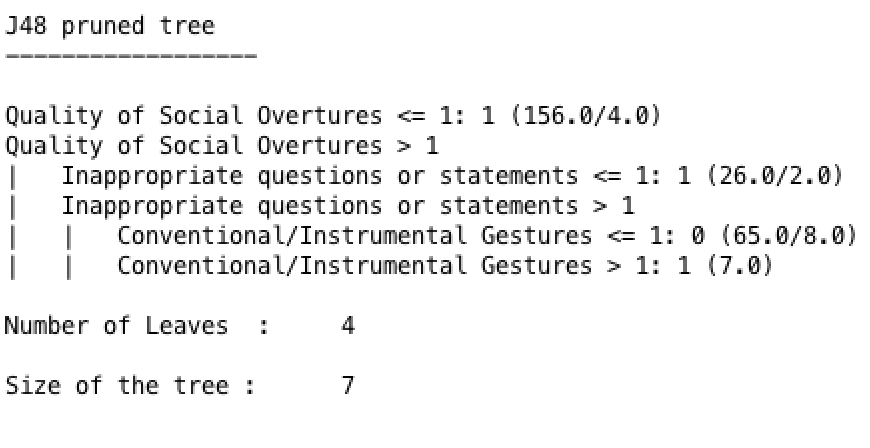
\includegraphics[width=0.6\textwidth]{Figures/Figure_5_1.png}}
  \caption{J48 pruned tree with ADI parent-oriented review}
  \label{fig:51}
\end{figure}

\begin{figure}
\centering
  {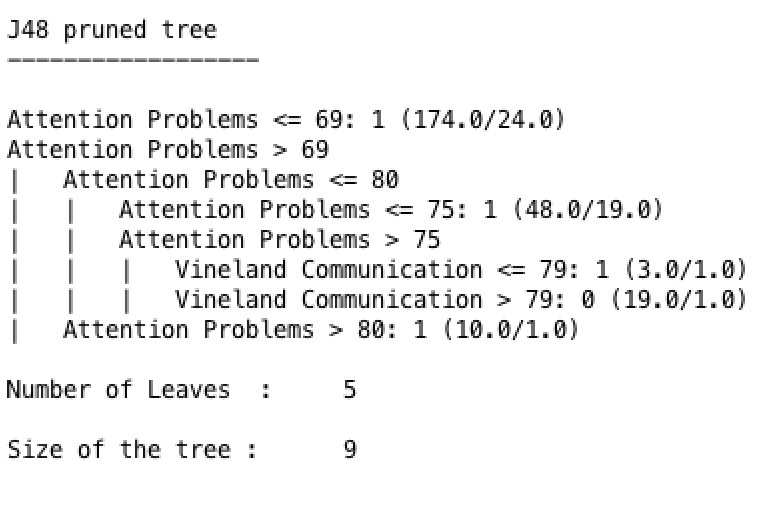
\includegraphics[width=0.6\textwidth]{Figures/Figure_5_2.png}}
  \caption{J48 pruned tree with BASC and VINE parent-oriented review}
  \label{fig:52}
\end{figure}

\subsection{Individual Feature Sets Analysis}
As the date consists of four different types of features, Random Forest model is trained on each of these feature sets. The four different feature sets are IQ, ADI BASC and VINE feature set. The results of these Random Forest models are obtained in table \ref{table:55}. When analyzing the IQ feature set, additional data from the ABIDE and ADHD-200 dataset was taken. The subjects from these datasets were taken by random sampling strategy. So, when the Random Forest model was trained on these there groups of data(ASD, ADHD, ASD+ADHD), the performance of the model dropped. It had an accuracy of 60\% which is lesser compared to the IQ feature set analysis of groups(ASD, ASD+ADHD). Therefore, from the models obtained, IQ of the child is not a clear indicator of the diagnosis of the child, that is the ASD and ADHD comorbidity cannot be analyzed with IQ.

\begin{table}[h]
\begin{center}
\begin{tabular}{|l|c|c|c|c|}
\hline
\textbf{Feature Set} & \textbf{Accuracy(\%)}&	\textbf{Precision(\%)}&	\textbf{Recall(\%)}&	\textbf{ROC Area}\\
\hline \hline
IQ	&65.7\%	 &0.628 &	0.657&	0.588\\
\hline
ADI& 96\% &	0.960 &	0.961 &	0.966\\
\hline
BASC &75.98\%	&0.726	&0.760	&0.727\\
\hline
VINE&	73.6\%	&0.562 &	0.736 &	0.557\\
\hline
\end{tabular}
\end{center}
\caption{Random Forest algorithm with different feature sets.}
\label{table:55}
\end{table}

By analyzing the models, it can be seen that ADI parent-oriented review is performing better than the other three feature sets. Similar results were obtained when analyzing the feature selection models. Therefore, for distinguishing the two groups ADI parent-oriented review plays a vital and only this review could be used to diagnose the children as well.

\subsection{Ensemble methods to predict ADHD in Autistic children}
Ada Boosting and Logit Boosting are two different types of boosting techniques that have been used on our data. Ada Boost uses weights to give more importance to certain variables over others. It is an iterative method that classifies data in the best way possible at each step. Logit Boosting also works similar to Ada Boost however, the cost function through which weights are given to variables varies in both these algorithms. For logit boosting the cost function is of that applied to logistic regression and minimizes the logistic loss in (1) and the training error function minimized by Ada boosting algorithm at each iteration t is given in (2).
$$
\sum_{i} \log (1+e^{-y_{i}f(x_{i})})\eqno{(1)}
$$

$$
\sum_{i} E[F_{t-1}(x_{i})+ \alpha_{t}h(x_{i})] \eqno{(2)}
$$
The Ada Boosting technique took 5 iterations and the accuracy of the model is 90.5\% while the ROC Area is 0.951. Also, the precision and recall for ASD+ADHD group is 76\% and 92\% and for the ASD group is 97\% and 90\%. The features selected by the Ada Boosting algorithm at each iteration are given below:
\begin{compactenum}
\item Quality of social overtures- According to Ada Boosting if the value of this feature is equal to 2, then with 60\% confidence the class is ASD+ADHD. However, when the feature value is not equal to 2, then with 97\% confidence it is ASD. This was selected in the first iteration with weight of 1.59.
\item Attention Problems- When the subjects feature value is greater than 69.5 than it belongs to ASD class with 52\% confidence, but it has higher confidence of 92\% when it is less than or equal to 69.5. This was selected in iteration 2 and 4 with weights of 1.47 and 1.24 respectively.
\item Offering to share- When the subjects feature value is not equal to 1 than it belongs to class ASD+ADHD with 63\% confidence. On the other hand, when feature value is equal to 1, then it belongs to ASD class with 97\% accuracy. This was selected in iteration 3 with weight of 0.9.
\item Inappropriate questions or statements- When the subjects feature value is not equal to 2 than it belongs to class ASD with 87\% confidence. However, when feature value is equal to 2, then it belongs to ASD+ADHD class with 66\% accuracy. This was selected in iteration 3 5 with weight of 1.18.
\end{compactenum}

Similarly, when Logit Boosting technique has been applied to the data, the accuracy of the model is 92\% and the ROC Area is 0.949. The precision and recall for the ASD class is 94\% each. On the other hand, the precision and recall for the ASD+ADHD class is 84\% each. The features selected by Boosting technique at each iteration is given below:
\begin{compactenum}
\item Quality of social overtures
\item Inappropriate questions or statements
\item Attention Problems
\item Response to Approaches of other children
\item Conventional/Instrumental Gestures
\end{compactenum}

\subsection{Observations}
During the comparison of all the three feature selection algorithms, it can be seen that the variable “Vineland Socialization” of the VINE is most important over others as two of our feature selection algorithms have selected it. Similarly, “Attention Problems” variable from BASC and “Quality of social overtures” and “Inappropriate questions or statements” variables from ADI. These variables that our algorithm has selected are actually the most important signs of ASD and ADHD in individuals when compared to other signs.

The results obtained after applying boosting techniques show that rules can be made for these features in the form of decision stumps, which will help in better diagnosis. Also, Logit Boosting performed better with our data over Ada Boosting. The most important features that have been selected by majority of our machine learning algorithms are given below:
\begin{compactenum}
\item Quality of social overtures
\item Inappropriate questions or statements
\item Attention Problems
\item Conventional/Instrumental Gestures
\end{compactenum}

Our data doesn’t contain control groups, so the false diagnosis of these disorders was not a problem. But, even in the existing data false negatives of ADHD are minimal, this shows that machine learning is doing a good job at predicting if autistic children are showing signs of ADHD or not. It shows positive signs of being able to distinguish ASD patients from the ASD+ADHD patients with limited variables. These techniques could be applied to larger datasets and our models would be more generalized. Hence, even though these methods are not ready to be used in real-time, the results of our study indicate that in the near future, machine learning will show promising results in the clinical diagnosis of developmental disorders specifically those that do not have genetic relations like ASD and ADHD.

\section{VCFS and ASD Comorbidity}
When analyzing the comorbid disorders ASD and VCFS, the data has been separated for this purpose. It consists of subjects who are diagnosed with ASD, VCFS and both these disorders together. On this modifies data, different machine learning algorithms have been applied. Also, the features selected by different feature selection algorithms in chapter 3 are also used to build models. The observations made in this analysis are discussed in the next section.
\subsection{Applying Supervised Learning Techniques}

The data which consists of the three different class labels that is used for this analysis has already been preprocessed in the chapter 3, now this data is loaded into WEKA and different machine learning classifiers in WEKA are used to build our models. These algorithms have been applied to our data to build models as they are suitable for data and these algorithms work well with the type of data that we have. The results obtained from our machine learning algorithms on our data is given below in table \ref{table:56}. \nomenclature{SVM}{Support Vector Machine}
\begin{table}[h]
\begin{center}
\begin{tabular}{|l|c|c|c|c|}
\hline
\textbf{ML Algorithm} & \textbf{Accuracy(\%)}&	\textbf{Precision(\%)}&	\textbf{Recall(\%)}&	\textbf{ROC Area}\\
\hline \hline
Naive Bayes	&94.11&	0.953&	0.941&	0.994\\
\hline
Logistic Regression&	89.8	&0.902&	0.899&	0.963\\
\hline
Random Forest&96.7 &	0.968 &	0.967	&0.997\\
\hline
Support Vector Machine&97.0	&0.970&	0.971&	0.976\\
\hline
$K$ Nearest Neighbors ($n$=3)&93.7&	0.940&	0.938&	0.980\\
\hline
\end{tabular}
\end{center}
\caption{Supervised Learning techniques for ASD and VCFS comorbidity}
\label{table:56}
\end{table}

By comparing the different supervised learning techniques both SVM and Random Forest algorithms have similar model performance. Also, both these models are better than other machine learning techniques that have been used. When the models are compared based on each of the class labels, then SVMs are better than Random Forest. Using the entire features available for the data, the J48 algorithm summarized our model. The results obtained from our J48 algorithm are shown in figure \ref{figure:53} For further analysis of these comorbid disorders, SVM models are built on each of the features selected by the feature selection algorithms in chapter 3. The results obtained by these SVM models are shown in table \ref{table:57}.
\begin{figure}
\centering
  {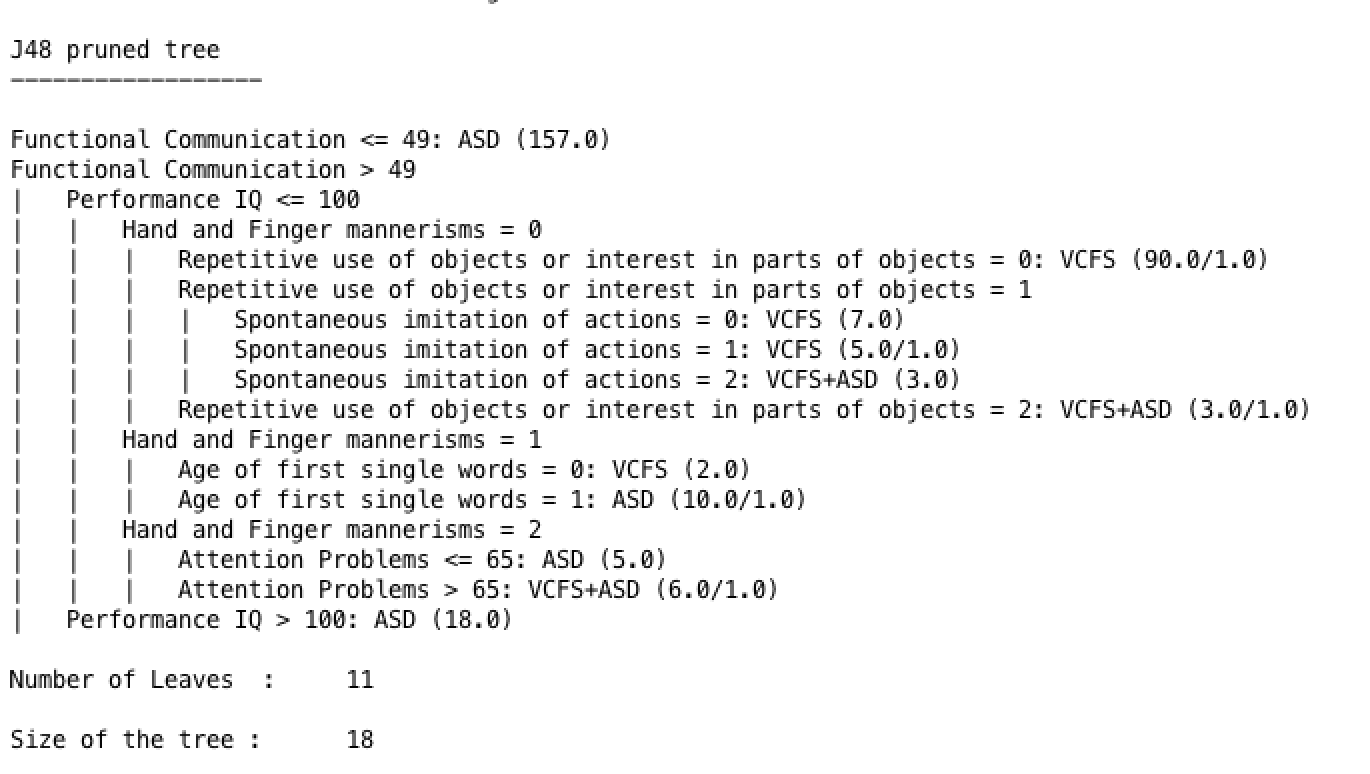
\includegraphics[width=0.6\textwidth]{Figures/Figure_5_3.png}}
  \caption{J48 pruned tree with ADI feature set}
  \label{fig:53}
\end{figure}
\begin{table}[h]
\begin{center}
\begin{tabular}{|l|c|c|c|c|}
\hline
\textbf{Feature Selection Algorithm}& \textbf{Accuracy(\%)}&	\textbf{Precision(\%)}&	\textbf{Recall(\%)}&	\textbf{ROC Area}\\
\hline \hline
LASSO&	62.09&	0.389&	0.621&	0.498\\
\hline
ReliefF&	78.43&	0.765&	0.784&	0.805\\
\hline
RFE&	90.5&	0.873&	0.905&	0.909\\
\hline
\end{tabular}
\end{center}
\caption{Feature Selection Algorithms for ASD and VCFS comorbidity}
\label{table:57}
\end{table}

SVM model trained by RFE features is the best and the performance of the other to models is not comparable to our previous models. If this model was compared to SVM model with entire dataset, it could be seen that the performance of the model has dropped by 7\%.

\subsection{Individual Feature Sets Analysis}
In this section, ASD and VCFS comorbidity is analyzed with respect to each of the individual feature sets present in our data. The SVM model which is performing well with our data is trained on each of the individual feature sets. The results of these models are shown in table \ref{table:58}. By comparing these models, ADI parent oriented reviews model performance is better than other feature sets. However, when compared to the previous models of SVM, the performance is less, but this model could be a better generalization of our data. 
\begin{table}[h]
\begin{center}
\begin{tabular}{|l|c|c|c|c|}
\hline
\textbf{Feature Set}& \textbf{Accuracy(\%)}&	\textbf{Precision(\%)}&	\textbf{Recall(\%)}&	\textbf{ROC Area}\\
\hline \hline
IQ	&63.07\%&	0.566&	0.631&	0.518\\
\hline
ADI& 93.13\%&	0.927&	0.931	&0.936\\
\hline
BASC &84.96\%&	0.841&	0.850&	0.874\\
\hline
VINE&	80.3\%&	0.785&	0.804&	0.825\\
\hline
\end{tabular}
\end{center}
\caption{Random Forest algorithm with different feature sets.}
\label{table:58}
\end{table}

\subsection{Applying Ensemble Methods}
Ada Boosting and Logit Boosting techniques were applied to the ASD and VCFS data and the performance of these models has been analyzed. The accuracy of Ada Boosting technique is 92.15\% and ROC Area is 0.978. The Ada model takes 5 iterations and the features selected at each iteration are given below:
\begin{compactenum}
\item Criteria for Repetitive behaviors and stereotyped patterns- When this feature value is equal to ‘Yes’, then child belongs to the class label ASD with 90\% confidence. However, when the feature value is not ‘Yes’, then child belong to class label VCFS  with 88\% confidence. The weight given to this feature is 2.18.
\item Functional Communication- The subject belongs to the class ASD, when the feature value is less than or equal to 49.5 with 100\% confidence. On the other hand, individuals belongs to class VCFS with less confidence of 54\%, if the feature value is greater than 49.5. The weight assigned to this feature is 1.08.
\item Adaptive Daily Living- The weight for this feature is 0.67. When this feature takes a value less than of equal to 49 subjects belongs to ASD class with 100\% confidence. However, when the value is greater than 49, with 50\% confidence the subjects belongs to the VCFS and ASD class.
\item Vineland Composite- The weight assigned for this feature is 0.4. The class label is VCFS with 42\% confidence, if the feature value is less than 98.5. Also, the class label is ASD with 97\% confidence, if feature value is greater than 98.5
\item Criteria for Communication- When this feature value is equal to ‘Yes’, then subject belongs to the class label VCFS+ASD with 50\% confidence. However, when the feature value is not ‘Yes’, then child belong to class label VCFS  with 64\% confidence. The weight given to this feature is 0.22.
\end{compactenum}
Logit Boosting has a model accuracy of 95.7\% and ROC Area value of .988. It is performing better than Ada boosting. Also, for subjects that both these disorders, the model performance is better. The features selected by Login Boosting are given below:
\begin{compactenum}
\item Functional Communication
\item Criteria for Repetitive behaviors and stereotyped patterns
\item Vineland Daily Living
\item Criteria for Qualitative impairments in reciprocal social interaction
\item Quality of social overtures
\item Adaptive Daily Living
\item Hyperactivity
\item Performance IQ
\item Criteria for Communication
\item Spontaneous imitation of actions
\item Attention Problems
\item Verbal IQ
\item Somatization
\end{compactenum}

\subsection{Observations}
As our data consists of less number of children who are diagnosed with VCFS and ASD, the models that are being trained on this data are able to precisely detect those children. However, it cannot be guaranteed that our models are able to generalize this class label.Our models are doing a good job with the individual diagnosis of ASD and VCFS especially the Support Vector Machine algorithm. The best features which help in analyzing our comorbid disorders are given below:
\begin{compactenum}
\item Functional Communication
\item Criteria for Communication
\item Spontaneous imitation of actions
\item Adaptive Daily Living
\item Criteria for Repetitive behaviors and stereotyped patterns
\item Repetitive use of objects or interest in parts of objects
\end{compactenum}

On comparison of the feature sets, ADI parent-oriented review is better than the other two parent-oriented reviews. Also, the IQ feature set is not good at analyzing the comorbidity of ASD and VCFS. Overall, due to the difference in the class proportions, the machine learning algorithms are not able to categorize when generally. Also, RFE has selected features from ADI parent-oriented reviews and it is better than other feature selection algorithms. When comparing the boosting techniques, Logit is doing better, but it has chosen a variety of features. Therefore, for analyzing ASD and VCFS comorbidity, ADI parent-oriented review provide better generalization and so does the J48 model.
\chapter{Investigating Developmental Disorders Diagnosis}
The target label of the data is modified to binary to examine the individual developmental disorders. After converting the label, each of the disorders are studied individually in this chapter. In the first section, ASD features and models are discovered, while in the second section, ADHD features and models are discovered. Finally, the last section VCFS features and models are built. Each of these sections help us understand these disorders and show results for children if these disorders existed exclusively in the children. This chapter discusses more specifically about their individual existence in the children. Also, impact of each of these individual parent-oriented reviews along with the IQ features on the developmental disorders will be discussed. Discussions are also done on the models that will we built for each of the developmental disorders using the features selected in chapter 3 by each of the feature selection algorithms.

\section{Austism Spectrum Disorder}
The target label diagnosis in the subgroup data has been modified to predict if a child has ASD or not. The data is modifies to understand and build models specific to ASD. This data will analyze ASD related features and models in greater depth. On this dataset different supervised learning techniques Logistic Regression, Decision Trees, K-Nearest Neighbors and Random Forest have been applied from the sklearn package in python and the following is the ROC curves obtained in figure \ref{fig:61}. The metrics for evaluation of these techniques are given in the table \ref{table:61}.
%table 6.1
\begin{table}[t]
\begin{center}
\begin{tabular}{|l|c|c|}
\hline
\textbf{ML Algorithm} & \textbf{Accuracy}&	\textbf{ROC Area}\\
\hline \hline
Random Forest&	98.64\%&	0.99137\\
\hline
Logistic Regression&	98.64\%&	0.96875\\
\hline
$K$- Nearest Neighbors($n$=3)&	85.135\%&	0.79202\\
\hline
Decision Tree&	97.297\%&	0.9375\\
\hline
\end{tabular}
\end{center}
\caption{ Supervised learning techniques comparison based on different metrics for ASD }
\label{table:61}
\end{table}

Among these supervised learning model, Random forest seems to be better fitting the `ASD data` when compared to other models. It has better Area Under Curve value than Logistic Regression model, even though the accuracy is same. By analyzing the results, it can be observed that tree based algorithms are doing a good job and the model for examining ASD can be repressed in the form of a tree. So, J48 algorithm is applied to describe the tree for our data, which can be seen in figure \ref{fig:62}.
\begin{figure}
\centering
  {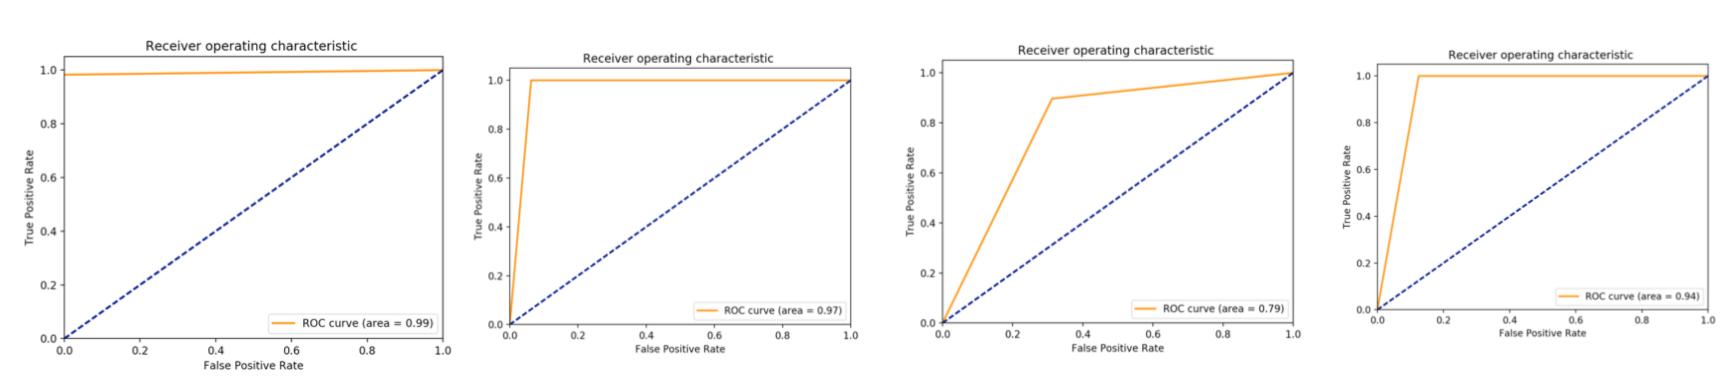
\includegraphics[width=0.8\textwidth]{Figures/Figure_6_1.png}}
  \caption{ ROC curve for ASD dataset \\a) Random Forest b) Logistic Regression c) KNN(n=3) d) Decision Tree }
  \label{fig:61}
\end{figure}
The accuracy of J48 algorithm is 96\% and ROC Area is 0.96. Also, for each individual group, the precision and recall are good. By combining the precision and recall, it can be seen that the F-measure for ASD subjects is 97\% and the F-measure for non-ASD subjects is 93\%. This shows that J48 is doing a good job at summarizing the results of the ASD data.


When training the Random Forest model, based on the features selected in chapter 3, table 6.2 shows the results of each of the feature selection algorithm. The features selected by ReliefF and RFE are performing better than the features selected by LASSO. The features selected by RFE is from the ADI parent-oriented review and hence, the ADI parent oriented review seems to be building better models when compared to the other parent oriented reviews.
\begin{figure}
\centering
{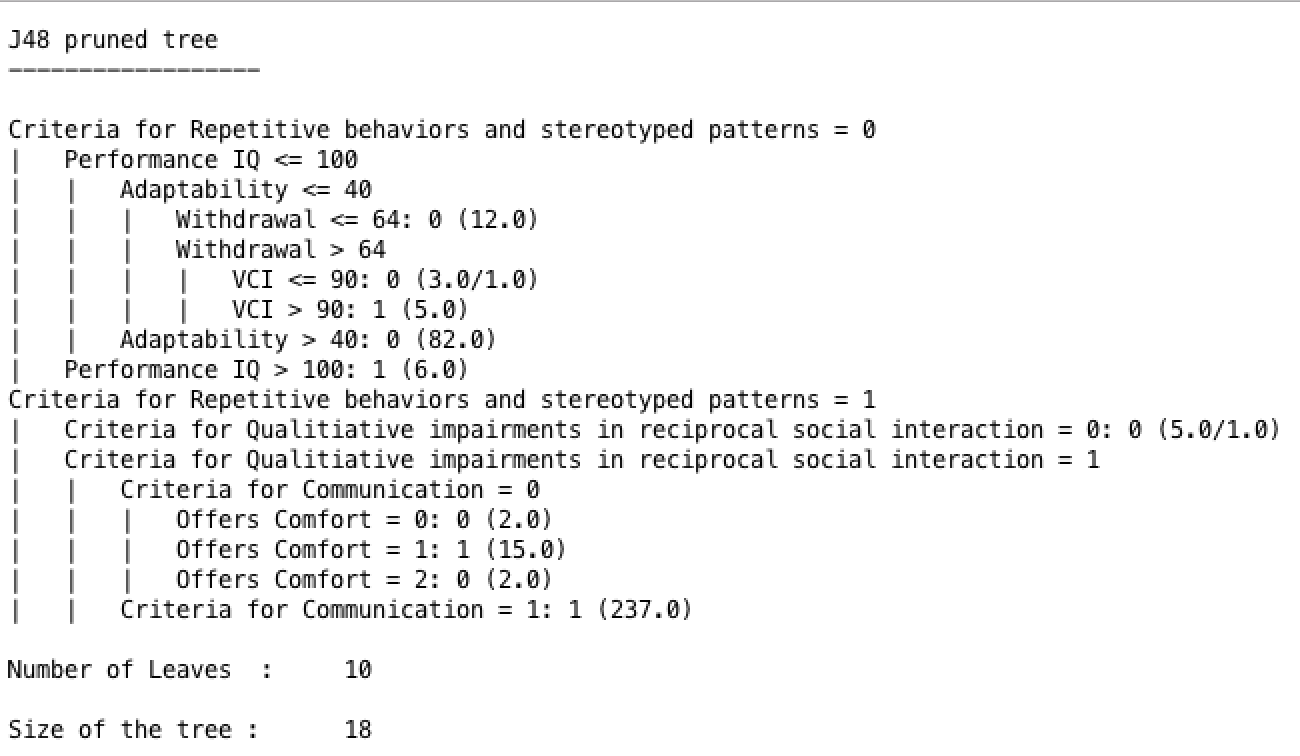
\includegraphics[width=0.6\textwidth]{Figures/Figure_6_2.png}}
  \caption{ J48 pruned tree for ASD  }
  \label{fig:62}
\end{figure}
%table 6.2
\begin{table}[h]
\begin{center}
\begin{tabular}{|l|c|c|c|}
\hline
\textbf{Feature Selection Algorithm}&	\textbf{Accuracy}&	\textbf{F-measure}&	\textbf{ROC Area}\\
\hline \hline
LASSO	&82.6 &	0.824	& 0.898\\
\hline
ReliefF &	91.3&	0.915&	0.967\\
\hline
RFE &	95.3 &	0.954 &	0.959\\
\hline
\end{tabular}
\end{center}
\caption{ Random Forest model trained with Feature Selection Algorithms for ASD }
\label{table:62}
\end{table}

\subsection{Predicting Diagnosis based on IQ feature set}
Based on the IQ features, different supervised learning techniques (random Forest, Naive Bayes, Logistic Regression) have been applied to predict ASD diagnosis for given dataset. These algorithms are used from WEKA by loading this data into it. The table \ref{table:63} shows the various metrics based on which the techniques are evaluated.
%table 6.3
\begin{table}[h]
\begin{center}
\begin{tabular}{|l|c|c|c|c|c|}
\hline
\textbf{ML Technique}&	\textbf{Precision}&	\textbf{Recall}&	\textbf{F-measure}&	\textbf{ROC Area}&	\textbf{Accuracy}\\
\hline \hline
Random Forest&	0.878&	0.878&	0.878&	0.930&	87.80\%\\
\hline
Naive Bayes&	0.693&	0.688&	0.691&	0.686&	68.83\%\\
\hline
Logistic Regression	&0.683&	0.713&	0.689&	0.796&	71.273\%\\
\hline
\end{tabular}
\end{center}
\caption{Supervised Learning Techniques applied on IQ features/variables for ASD }
\label{table:63}
\end{table}

Random Forest supervised learning technique is good at predicting ASD based on the IQ scores of the children with an accuracy of 87.8\%. The accuracy for model has dropped from 96\% as the features have been reduced to only IQ features. In comparison, it can be said that IQ features are not doing well compared to the entire feature set, so IQ feature set only is not a suitable method for predicting if a child has ASD or not.

\subsection{Predicting Diagnosis based on ADI feature set}
Further analysis has been done based on the ADI features, different supervised learning techniques have been applied to predict ASD diagnosis for given dataset. The table \ref{table:64} below shows the various metrics based on which the supervised learning techniques are evaluated.
%table 6.4
\begin{table}[h]
\begin{center}
\begin{tabular}{|l|c|c|c|c|c|}
\hline
\textbf{ML Technique}&	\textbf{Precision}&	\textbf{Recall}&	\textbf{F-measure}&	\textbf{ROC Area}&	\textbf{Accuracy}\\
\hline \hline
Random Forest&0.968&	0.967&	0.968&	0.991	&96.74\%\\
\hline
Naive Bayes&	0.948&	0.949&	0.948&	0.960&	94.85\%\\
\hline
Logistic Regression	&0.918&	0.916&	0.917	&0.954&	91.59\%\\
\hline
\end{tabular}
\end{center}
\caption{Supervised Learning Techniques applied on ADI feature set for ASD}
\label{table:64}
\end{table}

Random Forest supervised learning technique is good at predicting ASD based on the ADI feature/ variable scores of the children. Also, the ADI review is specifically designed for finding ASD behaviors in a child and hence, most models have high accuracy along with high ROC values. The accuracy of this model is similar to that of the J48 model and hence, ADI feature set could be used individually to diagnose a child with ASD.

\subsection{Predicting Diagnosis based on BASC feature set}
Based on the BASC feature set, different supervised learning techniques have been applied to predict ASD diagnosis for given dataset. The table \ref{table:65} shows the various metrics based on which the techniques are evaluated.
%table 6.5
\begin{table}[h]
\begin{center}
\begin{tabular}{|l|c|c|c|c|c|}
\hline
\textbf{ML Technique}&	\textbf{Precision}&	\textbf{Recall}&	\textbf{F-measure}&	\textbf{ROC Area}&	\textbf{Accuracy}\\
\hline \hline
Random Forest&0.920	&0.908&	0.910	&0.965&	90.78\%\\
\hline Naive Bayes&	0.915&	0.892&	0.895&	0.928&	89.15\%\\
\hline
Logistic Regression	&0.879	&0.875&	0.877	&0.936&	87.53\%\\
\hline
\end{tabular}
\end{center}
\caption{Supervised Learning Techniques applied on BASC feature set for ASD}
\label{table:65}
\end{table}

Random Forest supervised learning technique is good at predicting ASD based on the BASC feature scores of the children with an accuracy of 90.78\%. Even though the model accuracy has dropped to 91\% when compared to the J48 model, BASC features could still be used to predict if a child has ASD or not.

\subsection{Predicting Diagnosis based on VINE feature set}
Based on VINE feature set, different supervised learning techniques from WEKA have been applied to predict ASD diagnosis for given dataset. The table \ref{table:66} shows the various metrics based on which the techniques are evaluated. Random Forest and Logistic Regression supervised learning techniques are good at predicting ASD based on the VINE feature scores of the children with an accuracy of 88\%. However, the performance of both these models is less than 10\% when compared tot he J48 model and the model with ADI features. 
%table 6.6
\begin{table}[h]
\begin{center}
\begin{tabular}{|l|c|c|c|c|c|}
\hline
\textbf{ML Technique}&	\textbf{Precision}&	\textbf{Recall}&	\textbf{F-measure}&	\textbf{ROC Area}&	\textbf{Accuracy}\\
\hline \hline
Random Forest&0.884	&0.881&	0.882&	0.941&	88.07\%\\
\hline
Naive Bayes&0.792	&0.786	&0.788	&0.869&	78.59\%\\
\hline
Logistic Regression	&0.885&	0.883&	0.884&	0.917&	88.34\%\\
\hline
\end{tabular}
\end{center}
\caption{Supervised Learning Techniques applied on VINE feature set for ASD }
\label{table:66}
\end{table}

On the other hand, even though the model with VINE features is not doing well, it is better than the model with IQ features. So, only the VINE parent-oriented features cannot be used to diagnose a child with ASD.

\subsection{Observations}
When diagnosing a child with ASD, it can be seen that tree-based machine learning techniques like Random Forest and J48 are doing well. Also, it possible to diagnose a child with ASD using ADI and BASC parent-oriented review, but ADI parent-oriented review seems to be performing better than both the other parent oriented reviews. This could also be seen as the RFE feature selection algorithm in chapter 3, selects features from the ADI parent-oriented review and that is the best model from our feature selection models. The important features selected by the J48 model are a combination of all three parent-oriented reviews and are given below:
\begin{compactenum}
\item Offers Comfort
\item Criteria for Qualitative impairments in reciprocal social interaction
\item Criteria for Communication
\item Criteria for repetitive behaviors and stereotyped patterns
\item Adaptability
\item Withdrawal
\item Performance IQ 
\end{compactenum}

The features selected from the different feature selection algorithms in chapter 3 are compared to these features and 3 out of 7 of these features are same. It can be seen that J48 is converging the features selected by each of those algorithms. On an average, all the models to predict ASD have an accuracy of 90\%. The model with highest accuracy is with ADI parent-oriented review features. Therefore, it is observed that rather than using all the features in the data given, only the features of ADI parent-oriented reviews are sufficient, this supports the fact that ADI parent-oriented review is used to diagnose children with ASD.

\section{Attention Deficit/Hyperactivity Disorder}
The target label diagnosis in the subgroup data has been modified to predict if a child has ADHD or not. The dataset being used for this is converted, that is the class label is modified. On this dataset different supervised learning techniques Logistic Regression, Decision Trees, Naive Bayes and Random Forest have been applied and the following is the ROC curves obtained in figure \ref{figure:63}. The metrics for evolution of these techniques are given in the table \ref{table:67}.

%table 6.7
\begin{table}[h]
\begin{center}
\begin{tabular}{|l|c|c|}
\hline
\textbf{ML Algorithm }& \textbf{Accuracy}&	\textbf{ROC Area}\\
\hline \hline
Random Forest&	95.945\%&	0.90625\\
\hline
Logistic Regression&	77.027\%&	0.604525\\
\hline
$K$- Nearest Neighbors($n$=3)&	79.792\%	&0.8028\\
\hline
Decision Tree&	93.24\%&	0.8890\\
\hline
\end{tabular}
\end{center}
\caption{Supervised learning techniques based on different metrics for ADHD }
\label{table:67}
\end{table}

\begin{figure}
\centering
  {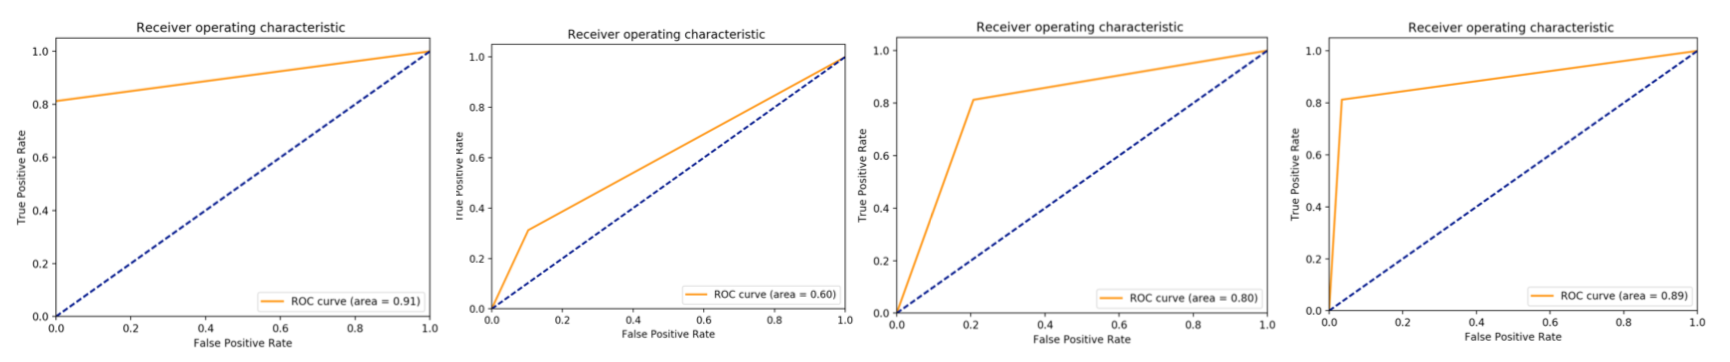
\includegraphics[width=0.8\textwidth]{Figures/Figure_6_3.png}}
  \caption{ ROC curve for ADHD dataset \\ a) Random Forest b) Decision Tree c) Naive Bayes d) Logistic Regression }
  \label{fig:63}
\end{figure}

Among these supervised learning models, Random Forest seems to be better fitting the `ADHD dataset` when compared to other models. It has better Area Under Curve value and accuracy. As the Random Forest is doing well for ADHD data, the features selected by each of the feature selection algorithm are trained using the random forest model and the performance of these three model is given in table \ref{table:68}.
%table 6.8
\begin{table}[h]
\begin{center}
\begin{tabular}{|l|c|c|c|}
\hline
\textbf{Feature Selection Algorithm}&	\textbf{Accuracy}&	\textbf{F-measure}&	\textbf{ROC Area}\\
\hline \hline
LASSO	&82.9\%&	0.813&	0.806\\
\hline
ReliefF &78.3\%	&0.764&	0.722\\
\hline
RFE &	95.9\%	&0.959&	0.942\\
\hline
\end{tabular}
\end{center}
\caption{ Random Forest model trained with Feature Selection Algorithms for ADHD}
\label{table:68}
\end{table}

When comparing the performance of models trained with the features from the three feature selection algorithms, it can be seen that RFE is doing better than the other two. Even though BASc is more commonly used to diagnose children with ADHD, this shows that ADI features can also do a good job at recognizing children with ADHD. 

As the random forest is doing well, another tree-based algorithm J48 is used to summarize our model and the prunes tree obtained from J48 algorithm is given in figure\ref{fig:64}. The algorithm had an accuracy of 94\% and it was good at diagnosing if children had ADHD or not. The F-measure for diagnosing ADHD is 83\% and without ADHD is 97\%. Since our data has small percentage of children when compared to those with ADHD, it can be seen that 83\% is comparable. Also, since the negative diagnosis percentage is high, it means that our model is doing well with trawl negative and can certainly till if a children doesn't have ADHD with good accuracy.
\begin{figure}
\centering
  {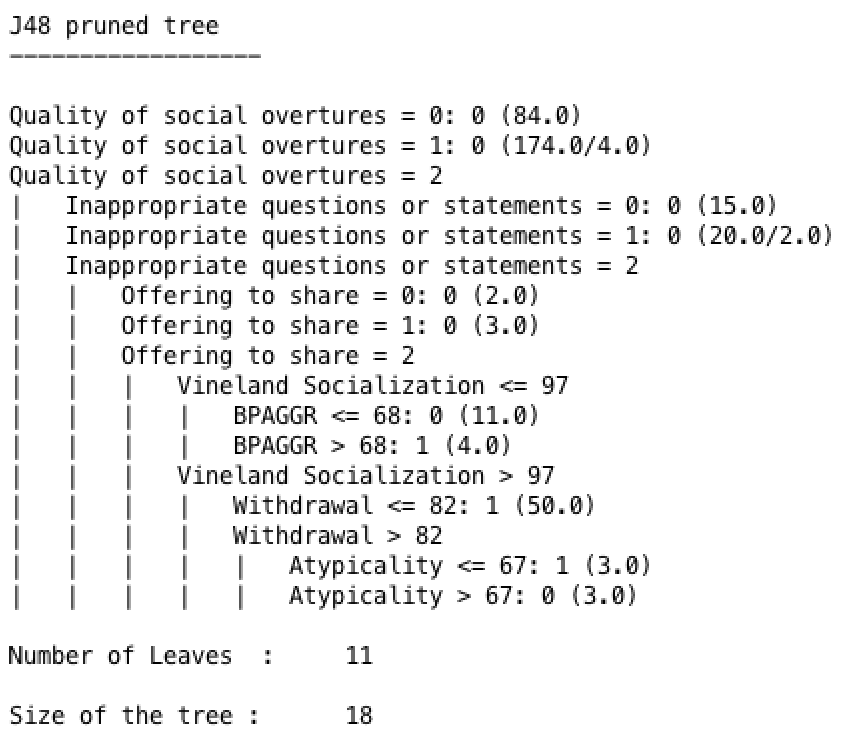
\includegraphics[width=0.6\textwidth]{Figures/Figure_6_4.png}}
  \caption{ J48 pruned tree for ADHD }
  \label{fig:64}
\end{figure}

\subsection{Predicting Diagnosis based on IQ feature set}
Based on the IQ feature set, different supervised learning techniques (Random Forest, Naive Bayes, Logistic Regression) have been applied to predict ADHD diagnosis for the modifies data. The table \ref{table:69} shows the various metrics based on which the techniques are evaluated.
%table 6.9
\begin{table}[h]
\begin{center}
\begin{tabular}{|l|c|c|c|c|c|}
\hline
\textbf{ML Technique}&	\textbf{Precision}&	\textbf{Recall}&	\textbf{F-measure}&	\textbf{ROC Area}&	\textbf{Accuracy}\\
\hline \hline
Random Forest&0.770&	0.799&	0.782&	0.714&	79.94\%\\
\hline
Naive Bayes&0.686	&0.818&	0.746	&0.556&	81.84\%\\
\hline
Logistic Regression	&0.792&	0.832&	0.772&	0.687&	83.19\%\\
\hline
\end{tabular}
\end{center}
\caption{Supervised Learning Techniques applied on IQ features/variables for ADHD  }
\label{table:69}
\end{table}

Logistic Regression supervised learning technique is good at predicting ADHD based on the IQ scores of the children. When comparing the performance of our model with the J48 model, it can be seen that the accuracy has dropped by 11\% and hence, only IQ features not sufficient at predicting if a child has ADHD.

\subsection{Predicting Diagnosis based on ADI feature set}
Now, further analysis is done based on the ADI feature set, different supervised learning techniques have been applied to predict ADHD diagnosis for modified data. The table \ref{table:610} shows the various metrics based on which the techniques are evaluated.
%table 6.10
\begin{table}[h]
\begin{center}
\begin{tabular}{|l|c|c|c|c|c|}
\hline
\textbf{ML Technique}&	\textbf{Precision}&	\textbf{Recall}&	\textbf{F-measure}&	\textbf{ROC Area}&	\textbf{Accuracy}\\
\hline \hline
Random Forest&0.981	&0.981	&0.981&	0.996	&98.10\%\\
\hline
Naive Bayes&0.934	&0.919&	0.923	&0.974	&91.86\%\\
\hline
Logistic Regression	&0.977&	0.976&	0.976&	0.687&	97.56\%\\
\hline
\end{tabular}
\end{center}
\caption{Supervised Learning Techniques applied on ADI features/variables for ADHD }
\label{table:610}
\end{table}

Random Forest supervised learning technique is good at predicting ADHD based on the ADI feature scores of the children and this also has high accuracy and ROC values for different classifier models. The Random Forest model with ADI feature set is better than the J48 model and Random Forest taking all the features into consideration. So, the J48 pruned tree using only the ADI features is given in figure 6.5. The accuracy of this model is 94.5\%, which is comparable to the previous J48 model. Also, the F-measure for diagnosing children with ADHD is 84.5\% which is more than our previous model diagnosis and for a children not having ADHD, the F-measure is 97\%. So, the ADI feature set is doing a better job at predicting if the child has ADHD better than the entire features of the data.
\begin{figure}
\centering
  {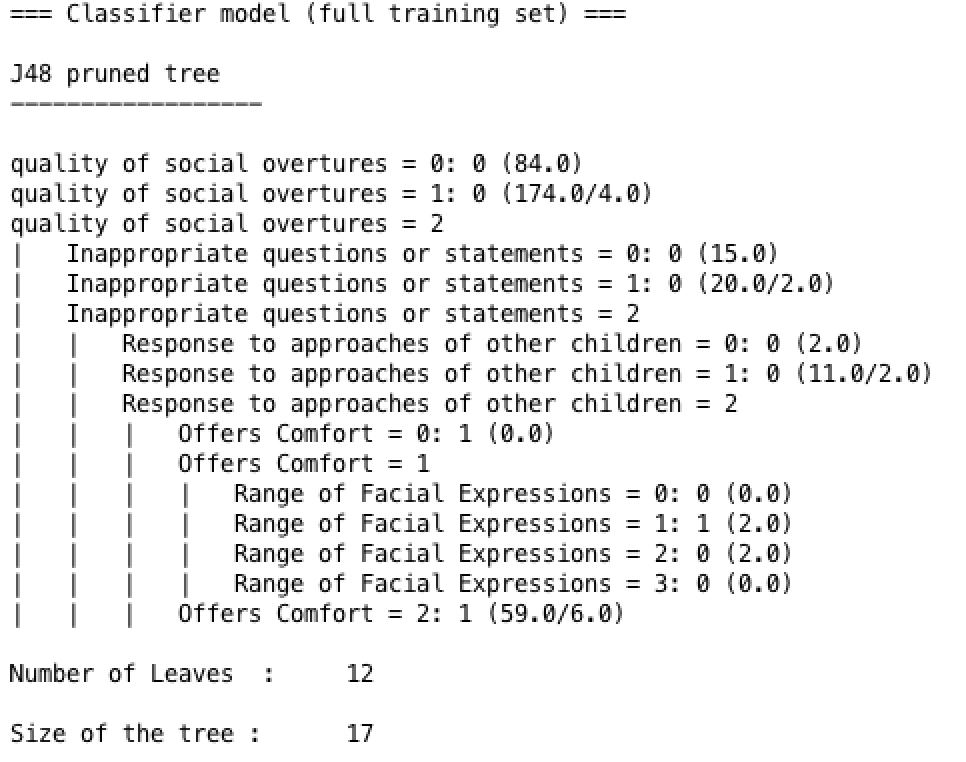
\includegraphics[width=0.8\textwidth]{Figures/Figure_6_5.png}}
  \caption{ J48 pruned tree for ADHD with ADI feature set}
  \label{fig:65}
\end{figure}

\subsection{Predicting Diagnosis based on BASC feature set}
Additional analysis is done using different supervised learning techniques to predict ADHD diagnosis for our converted data based on the BASC features/variables. The table \ref{table:611} shows the various metrics based on which the techniques are evaluated. Some of the supervised learning techniques applied from WEKA are Random Forest, Naive Bayes and Logistic Regression.
%table 6.11
\begin{table}[h]
\begin{center}
\begin{tabular}{|l|c|c|c|c|c|}
\hline
\textbf{ML Technique}&	\textbf{Precision}&	\textbf{Recall}&	\textbf{F-measure}&	\textbf{ROC Area}&	\textbf{Accuracy}\\
\hline \hline
Random Forest&0.794&	0.832&	0.793&	0.768&	83.19\%\\
\hline
Naive Bayes&0.792&	0.759&	0.773&	0.710&	75.88\%\\
\hline
Logistic Regression	&0.760&	0.802&	0.775&	0.709&	80.21\%\\
\hline
\end{tabular}
\end{center}
\caption{Supervised Learning Techniques applied on BASC features for ADHD }
\label{table:611}
\end{table}

Random Forest supervised learning technique is good at predicting ADHD based on the BASC scores of the children. However, when compared to the ADI model, our Random Forest classifier trains don BASC features has 10\% lower accuracy.

\subsection{Predicting Diagnosis based on VINE feature set}
Now, VINE features are applied to different supervised learning techniques to predict ADHD diagnosis for modifies data (target label modified to binary). The table \ref{table:612} shows the various metrics based on which the techniques are evaluated.

%table 6.12
\begin{table}[h]
\begin{center}
\begin{tabular}{|l|c|c|c|c|c|}
\hline
\textbf{ML Technique}&	\textbf{Precision}&	\textbf{Recall}&	\textbf{F-measure}&	\textbf{ROC Area}&	\textbf{Accuracy}\\
\hline \hline
Random Forest&0.685&	0.813&	0.744&	0.689&	81.30\%\\
\hline
Naive Bayes&0.851&	0.580&	0.627&	0.735	&57.9946\%\\
\hline
Logistic Regression	&0.687&	0.824&	0.749&	0.688&	82.38\%\\
\hline
\end{tabular}
\end{center}
\caption{Supervised Learning Techniques applied on VINE features for ADHD }
\label{table:612}
\end{table}

Logistic Regression supervised learning technique is good at predicting ADHD based on the VINE scores of the children. When the Logistic Regression model is compared to the ADI models, the performance of the model is not good, however, its performance is comparable to the model with BASC.
\subsection{Observations}
The analysis done in the above section shows that ADI parent-oriented review feature set is doing good at predicting if a child has ADHD. Moreover, our analysis shows that our models are good at eliminating true negatives that is there are better at diagnosing if the child doesn't have ADHD. The important ADI features, which can be used to diagnose a child with ADHD are given below:

\begin{compactenum}
\item Quality of social overtures
\item Inappropriate statements or questions
\item Group play with peers or friendships
\item Offers comfort
\item Response of approaches to other children
\item Range of facial expressions
\end{compactenum}

Most of these features selected were selected by our feature selection algorithms in chapter 3. Also, most of these features are important symptoms of diagnosing a child with ADHD.


\section{22Q Deletion Syndrome}
The target label diagnosis in the subgroup data has been modified into a binary attribute to predict if a child has ADHD or not. On this dataset different supervised learning techniques like Logistic Regression, Decision Trees, K-Nearest Neighbors and Random Forest have been applied and the following is the ROC curves obtained are present in figure\ref{fig:66}. These techniques have been applied from the sklearn package of python. The metrics for evaluation of these techniques are given in the table \ref{table:613}. 
%table 6.13
\begin{table}[h]
\begin{center}
\begin{tabular}{|l|c|c|}
\hline
\textbf{ML Algorithm} & \textbf{Accuracy}&	\textbf{ROC Area}\\
\hline \hline
Random Forest&	98.648\%&	0.99107\\
\hline
Logistic Regression&	97.297\%&	0.98214\\
\hline
$K$- Nearest Neighbors($n$=3)&91.891\%	&0.88988\\
\hline
Decision Tree&	83.7837\%&	0.79861\\
\hline
\end{tabular}
\end{center}
\caption{Supervised learning techniques based on different metrics for VCFS }
\label{table:613}
\end{table}

Among these supervised learning models, Random Forest seems to be better fitting the `VCFS dataset` when compared to other models, it has better Area Under Curve value and accuracy. Even Logistic Regression algorithm is fitting the data well and has a good accuracy of 97\%. Using the J48 algorithm, the pruned tree in figure \ref{fig:67} is a summarization of the model.
\begin{figure}
\centering
  {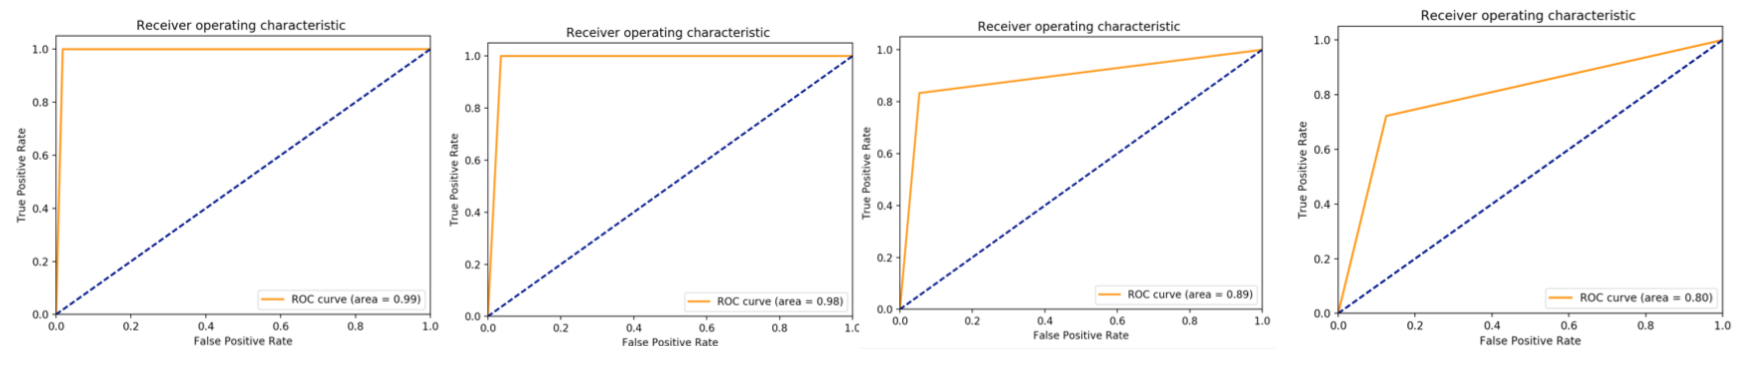
\includegraphics[width=0.8\textwidth]{Figures/Figure_6_6.png}}
  \caption{ ROC curve for VCFS dataset \\ a) Random Forest b) Decision Tree c) Naive Bayes d) Logistic Regression }
  \label{fig:63}
\end{figure}
\begin{figure}
\centering
  {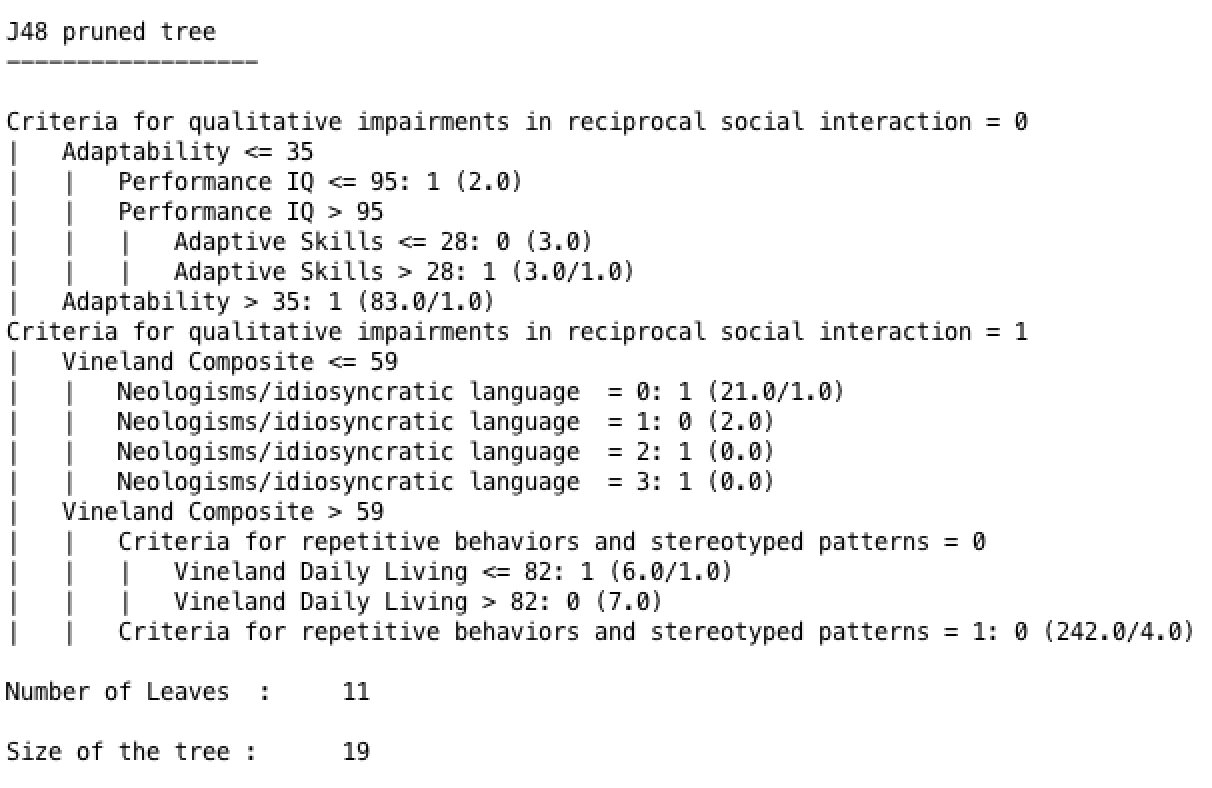
\includegraphics[width=0.8\textwidth]{Figures/Figure_6_7.png}}
  \caption{ J48 pruned tree for VCFS}
  \label{fig:67}
\end{figure}
The accuracy of this J48 is 93.4\%. The F-measure of diagnosing the children with VCFS is 90\% and the F-measure of not diagnosing the child with VCFS is 95.3\%. The performance of this model is not has good as the Random Forest model or Logistic Regression model, but it is comparable and a good way of representing our data. Now, the features selected in chapter 3 are used to train the Random Forest model as it is performing the best with our data and the results of the models for each feature selection algorithm are given in table \ref{table:614}. Among all the feature selection algorithms, LASSO is performing the best.
%table 6.14
\begin{table}[h]
\begin{center}
\begin{tabular}{|l|c|c|c|}
\hline
\textbf{Feature Selection Algorithm}&	\textbf{Accuracy}&	\textbf{F-measure}&	\textbf{ROC Area}\\
\hline \hline
LASSO	&92.4\%&	0.924&	0.974\\
\hline
ReliefF &787.2\%&	0.873&	0.922\\
\hline
RFE &	90.2\%	&0.903&	0.951\\
\hline
\end{tabular}
\end{center}
\caption{ Random Forest model trained with Feature Selection Algorithms for VCFS}
\label{table:614}
\end{table}

\subsection{Predicting Diagnosis based on IQ feature set}
Based on the IQ feature set, different supervised learning techniques have been applied to predict VCFS diagnosis for given dataset. The table \ref{table:615} shows the various metrics based on which the techniques are evaluated.
%table 6.15
\begin{table}[h]
\begin{center}
\begin{tabular}{|l|c|c|c|c|c|}
\hline
\textbf{ML Technique}&	\textbf{Precision}&	\textbf{Recall}&	\textbf{F-measure}&	\textbf{ROC Area}&	\textbf{Accuracy}\\
\hline \hline
Random Forest&0.883&	0.883&	0.883&	0.948&	88.34\%\\
\hline
Naive Bayes&0.692&	0.694&	0.693&	0.712&	69.37\%\\
\hline
Logistic Regression	&0.747&	0.759&	0.746&	0.825&	75.88\%\\
\hline
\end{tabular}
\end{center}
\caption{Supervised Learning Techniques applied on IQ features/variables for VCFS}
\label{table:615}
\end{table}

Out of all the supervised learning techniques, Random Forest is the best at predicting VCFS for children. However, compared to the previous Random Forest and J48 model, the accuracy has dropped by 7\% and hence, predicting ADHD with only the IQ feature set is not a good idea.

\subsection{Predicting Diagnosis based on ADI feature set}
Based on the ADI review feature set, different supervised learning techniques have been applied to predict VCFS diagnosis for given dataset. The table \ref{table:616} shows the various metrics based on which the techniques are evaluated.
%table 6.16
\begin{table}[h]
\begin{center}
\begin{tabular}{|l|c|c|c|c|c|}
\hline
\textbf{ML Technique}&	\textbf{Precision}&	\textbf{Recall}&	\textbf{F-measure}&	\textbf{ROC Area}&	\textbf{Accuracy}\\
\hline \hline
Random Forest&0.943&	0.943&	0.942&	0.981&	94.30\%\\
\hline
Naive Bayes&0.913&	0.913&	0.913&	0.927&	91.32\%\\
\hline
Logistic Regression& 0.922&	0.921&	0.922&	0.943&	92.14\%\\
\hline
\end{tabular}
\end{center}
\caption{Supervised Learning Techniques applied on ADI feature set for VCFS}
\label{table:616}
\end{table}

ADI feature set is doing better than IQ feature set when diagnosing children with VCFS. The best learning technique is Random Forest, but the performance of this model is low when compared to the Random Forest model with the entire dataset. However, ADI parent-oriented review features could be used to predict if a child has VCFS.

\subsection{Predicting Diagnosis based on BASC feature set}
Based on the BASC review feature set, different supervised learning techniques(Random Forest, Logistic Regression, Naive Bayes) have been applied to predict VCFS diagnosis for given dataset. The table \ref{table:617} shows the various metrics based on which the techniques are evaluated. 
%table 6.17
\begin{table}[h]
\begin{center}
\begin{tabular}{|l|c|c|c|c|c|}
\hline
\textbf{ML Technique}&	\textbf{Precision}&	\textbf{Recall}&	\textbf{F-measure}&	\textbf{ROC Area}&	\textbf{Accuracy}\\
\hline \hline
Random Forest&0.956&	0.951&	0.952&	0.983&	95.12\%\\
\hline
Naive Bayes&0.927&	0.916&	0.918&	0.933&	91.59\%\\
\hline
Logistic Regression& 0.896&	0.894&	0.895&	0.954&	89.43\%\\
\hline
\end{tabular}
\end{center}
\caption{Supervised Learning Techniques applied on BASC feature set for VCFS}
\label{table:617}
\end{table}

Among the different supervised learning techniques for predicting VCFS, Random Forest supervised learning technique is good to predict based on the BASC feature/variable scores of the children with accuracy of 95\%. So, the BASC parent oriented review is better than the ADI parent oriented review for predicting VCFS.

\subsection{Predicting Diagnosis based on VINE feature set}
Based on the VINE review feature set, different supervised learning techniques{random Forest, Naive Bayes, Logistic Regression} have been applied to predict VCFS diagnosis for given dataset. These supervised learning techniques are applied from WEKA. The table \ref{table:618} shows the various metrics based on which the techniques are evaluated. 
%table 6.18
\begin{table}[h]
\begin{center}
\begin{tabular}{|l|c|c|c|c|c|}
\hline
\textbf{ML Technique}&	\textbf{Precision}&	\textbf{Recall}&	\textbf{F-measure}&	\textbf{ROC Area}&	\textbf{Accuracy}\\
\hline \hline
Random Forest&0.887&	0.886&	0.887&	0.961&	88.16\%\\
\hline
Naive Bayes&0.812&	0.808&	0.809&	0.897&	80.75\%\\
\hline
Logistic Regression&0.891&	0.892&	0.891&	0.928&	89.15\%\\
\hline
\end{tabular}
\end{center}
\caption{Supervised Learning Techniques applied on VINE feature set for VCFS}
\label{table:618}
\end{table}

Even in this case for predicting VCFS, Random Forest supervised learning technique is good to predict based on the VINE feature scores of the children with accuracy of 88\% as it has a better ROC value when compared with Logistic Regression which has an accuracy of 89\%. The performance of this model is comparable to the performance of the IQ feature set models, but its performance is lower than all other models. As the children who have taken VINE is only 47\%, the model performance is good in comparison and it could be more generalized than other models.

\subsection{Observations}
Tree-based machine learning algorithms particularly Random Forest algorithm is doing best for diagnosing children with VCFS. Among the four different feature sets, BASC parent oriented reviews are doing the best. Even the though the performance of BASC parent-oriented review is good and comparable, the model with the entire features is out performing all the other models. The best features in the pruned tree are a combination of all the four feature sets present in our data.  Also, the best features selected by the J48 algorithm are as follows:
\begin{compactenum}
\item Adaptability
\item Criteria for Qualitative impairments in reciprocal social interaction
\item Performance IQ
\item Adaptive skills
\item Vineland Composite
\item Neologisms/idiosyncratic language
\item Criteria for Repetitive behaviors and stereotyped patterns
\item Vineland Daily Living
\end{compactenum}
Out of the 8 features selected by J48 algorithm, 6 of them were selected by our feature selection algorithms. Hence, these features are important for diagnosing a child with VCFS and no individual feature set out of the four feature sets could be used to diagnose children with VCFS. However, these features have more importance over other features in the given data and a model trained with these features performs well for predicting VCFS in children.
\chapter{Conclusion}
%\addcontentsline{toc}{chapter}{Conclusion}
\thispagestyle{plainbottom}
Your Conclusions here.
During our research, the main problem that was trying to be solved was early intervention of developmental disorders. Researchers in the past have shown that machine learning is useful to diagnose children with various disorders. So, by applying different machine learning techniques, different models were built to diagnose different developmental disorders. Also, models were built to understand the co-occurrences of these disorders. Apart for this our research also focused on analyzing the importance of each reviews to the diagnose and more specifically features which are an indicators of these developmental disorders.

Among the various supervised learning techniques, most of the times Random Forest models performed exceptionally well with our data. On the other hand, for feature selection, RFE was able to select the important features from our feature set. The important findings from our analysis are as follows:

\begin{itemize}
\item Most of our models predict the diagnosis labels in the subgroup data for male children with a better accuracy of 7\% when compared to female children. 
\item IQ features predict subgroup data diagnosis with 66.32\%, diagnose ASD with 87.8\%, diagnose ADHD with 83.19\% and diagnose VCFS with 88\% accuracy. Overall, IQ cannot be used to diagnose the subgroup data, but it could help with diagnosing ASD, ADHD and VCFS separately. 
\item BASC features predict subgroup data with 75\%, diagnose ASD with 90\%, diagnose ADHD with 83\% and diagnose VCFS with 95\% accuracy. These tests have a low prediction rate when compared to other tests for predicting the diagnosis of the subgroup data. 
\item VINE features predict subgroup data with 69\%, diagnose ASD with 88\%, diagnose ADHD with 82\% and diagnose VCFS with 89\% accuracy. This has the least accuracy values when compared to other tests, the main reason behind this could be that the number of children who have taken VINE test is less when compared to other two tests and the features of this VINE test is less when compared to the rest two tests. 
\item ADI review features predict subgroup data with 96.47\%, diagnose ASD with 96\%, diagnose ADHD with 98\% and diagnose VCFS with 94\% accuracy. ADI review test is better in predicting the diagnosis labels of subgroup data when compared to both the other tests. 
\item The comorbid disorders ASD and ADHD could be identified with ADI parent oriented reviews and there exist some important features on which the models achieved an average accuracy of  94\%.
\item Models could identify ASD and VCFS individually, but identifying their co-occurrence was more complex. The models built for ASD and VCFS comorbidity had an average accuracy of 90\%.
\item When comparing the individual diagnosis of children, it could be seen that predicting VCFS (98\%) among children with given features is better when compared to ASD and ADHD. Also, when clustering the children into different groups, the children diagnosed with VCFS were clustered appropriately (100\%) when compared to the ASD cluster. 
\end{itemize}

Our analysis shows machine learning is good at identifying these developmental disorders and they can help clinicians in diagnosing children with these orders. The models that have been found can also bee used to better emphasis on features more closely related to this developmental disorders. As our models identify comorbidity as well, these models would better assist clinicians when diagnosing children with multiple disorders.

The results and observations made in this research are a step towards using machine learning models to diagnose developmental disorders. Further analysis in this field will help us avoid confusions between different parent-oriented reviews and help us in justifying the importance of certain features over others during diagnosis. In the future, more studies could work on developing diagnostic specific models that will assess the disorder in children and their co-occurrences as well in an efficient and swift manner.



\bookmarksetup{startatroot}% this is it
\addtocontents{toc}{\bigskip}% perhaps as well


\bookmarksetup{startatroot}% this is it
\addtocontents{toc}{\bigskip}% perhaps as well

\backmatter
% put back links to the referencing page? http://tex.stackexchange.com/questions/36307/formatting-back-references-in-bibliography 
%\bibliography{thesis}{}
%\bibliographystyle{plain-annote}
%\bibliographystyle{jgsty}

\pagestyle{plain}
\printbibliography[heading=bibintoc]
\cleardoublepage

% an index? http://en.wikibooks.org/wiki/LaTeX/Indexing

\pagestyle{empty}
\cleardoublepage
\include{cv}
\end{document}

